\documentclass[8pt]{article}
\usepackage[margin=0.8in]{geometry}
\usepackage[utf8x]{inputenc}
\usepackage[T1]{fontenc}
\usepackage{listings}
\usepackage[dvipsnames]{xcolor}
\usepackage{amsthm}
\usepackage{graphicx}
\usepackage[most]{tcolorbox}
\usepackage{algorithm2e}

\begin{document}

\section{Information Measures}
\subsection{Independence and Markov Chain}
\begin{tcolorbox}
\paragraph{Definition 2.1 (Independence)} Two random variables $X$ and $Y$ are independent, denoted by $X \perp Y,$ if
$$
p(x, y)=p(x) p(y)
$$
for all $x$ and $y$ (i.e., for all $(x, y) \in \mathcal{X} \times \mathcal{Y})$.
\end{tcolorbox}

\begin{figure}[!h]
    \centering
    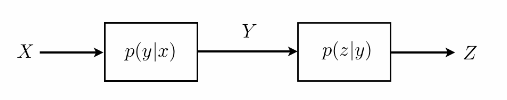
\includegraphics[width=0.5\linewidth]{imgs/def2_4.png}
    \caption{Conceptually, when $X \perp Z \mid Y$, $X, Y, Z$ are related as above.}
    \label{fig:my_label}
\end{figure}
\begin{tcolorbox}
\paragraph{Definition 2.2 (Mutual Independence)} For $n \geq 3,$ random variables $X_{1}, X_{2}, \cdots, X_{n}$ are mutually independent if, for all $x_{1}, x_{2}, \cdots, x_{n}$
$$
p\left(x_{1}, x_{2}, \cdots, x_{n}\right)=p\left(x_{1}\right) p\left(x_{2}\right) \cdots p\left(x_{n}\right)
$$
\paragraph{Definition 2.3 (Pairwise Independence)} For $n \geq 3,$ random variables $X_{1}, X_{2}, \cdots, X_{n}$ are pairwise independent if $X_{i}$ and $X_{j}$ are independent for all $1 \leq i<j \leq n$
\\
\paragraph{Definition 2.4 (Conditional Independence)} For random variables $X, Y$, and $Z, X$ is independent of $Z$ conditioning on $Y,$ denoted by \textcolor{blue}{$X \perp Z \mid Y$}, if
$$
p(x, y, z)=\left\{\begin{array}{cc}
\frac{p(x, y) p(y, z)}{p(y)}=p(x, y) p(z \mid y) & \text { if } p(y)>0 \\
0 & \text { otherwise }
\end{array}\right.
$$

\paragraph{Proposition 2.5} For random variables $X, Y,$ and $Z, X \perp Z \mid Y$ if and only if
$$
p(x, y, z)=a(x, y) b(y, z)
$$
for all $x, y,$ and $z$ such that $p(y)>0$

\end{tcolorbox}

\paragraph{Proof A.} `Only if' part. Assume $p(x, y, z)$ takes the form in Definition 2.4. For all $x$ and for all $y$ such that $p(y)>0,$ let
$$
a(x, y)=\frac{p(x, y)}{p(y)}
\quad \quad
b(y, z)=p(y, z)
$$
\paragraph{Proof B.} `If' part.\\
1. Assume that for all $x, y,$ and $z$ such that $p(y)>0$,
$$
p(x, y, z)=a(x, y) b(y, z)
$$
2. Then for such $x, y,$ and $z,$ we have
$$
p(x, y) =\sum_{z} p(x, y, z) =\sum_{z} a(x, y) b(y, z) =a(x, y) \sum_{z} b(y, z)
$$
$$
p(y, z) =\sum_{x} p(x, y, z) =\sum_{x} a(x, y) b(y, z) =b(y, z) \sum_{x} a(x, y)
$$
3. Furthermore,
$$
p(y)=\sum_{z} p(y, z)=\left(\sum_{x} a(x, y)\right)\left(\sum_{z} b(y, z)\right)>0
$$
4. Therefore,
$$
\frac{p(x, y) p(y, z)}{p(y)} =
\frac{\left(a(x, y) \sum_{z} b(y, z)\right) \left(b(y, z) \sum_{x} a(x, y)\right)}{
\left(\sum_{x} a(x, y)\right)\left(\sum_{z} b(y, z)\right)}
= a(x, y) b(y, z) =  p(x, y, z)
$$
5. And for $x, y,$ and $z$ such that $p(y)=0,$ since
$$
0 \leq p(x, y, z) \leq p(y)=0 \quad
\rightarrow \quad
p(x, y, z)=0
$$

\begin{tcolorbox}
\paragraph{Definition 2.6 (Markov Chain)} For random variables $X_{1}, X_{2}, \cdots, X_{n},$ where $n \geq 3, X_{1} \rightarrow X_{2} \rightarrow \cdots \rightarrow X_{n}$ forms a Markov chain if
$$
\begin{array}{l}
p\left(x_{1}, x_{2}, \cdots, x_{n}\right)= 
\left\{\begin{array}{ll}
p\left(x_{1}, x_{2}\right) p\left(x_{3} \mid x_{2}\right) \cdots p\left(x_{n} \mid x_{n-1}\right) & \text { if } p\left(x_{2}\right), p\left(x_{3}\right), \cdots, p\left(x_{n-1}\right)>0 \\
0 & \text { otherwise }
\end{array}\right.
\end{array}
$$
\paragraph{Remark.} \textcolor{blue}{$X_{1} \rightarrow X_{2} \rightarrow X_{3}$ is equivalent to $X_{1} \perp X_{3} \mid X_{2}$}
\\
\paragraph{Proposition 2.7} $X_{1} \rightarrow X_{2} \rightarrow \cdots \rightarrow X_{n}$ forms a Markov chain if and only if 
$X_{n} \rightarrow X_{n-1} \rightarrow \cdots \rightarrow X_{1}$ forms a Markov chain.
\\
\paragraph{Proposition 2.8} $X_{1} \rightarrow X_{2} \rightarrow \cdots \rightarrow X_{n}$ forms a Markov chain if and only if
$$
\begin{array}{l}
X_{1} \rightarrow X_{2} \rightarrow X_{3} \\
\left(X_{1}, X_{2}\right) \rightarrow X_{3} \rightarrow X_{4} \\
\qquad \qquad \vdots \\
\left(X_{1}, X_{2}, \cdots, X_{n-2}\right) \rightarrow X_{n-1} \rightarrow X_{n}
\end{array}
$$
form Markov chains.
\\
\paragraph{Proposition 2.9} $X_{1} \rightarrow X_{2} \rightarrow \cdots \rightarrow X_{n}$ forms a Markov chain if and only if
$$
p\left(x_{1}, x_{2}, \cdots, x_{n}\right)=f_{1}\left(x_{1}, x_{2}\right) f_{2}\left(x_{2}, x_{3}\right) \cdots f_{n-1}\left(x_{n-1}, x_{n}\right)
$$
for all $x_{1}, x_{2}, \cdots, x_{n}$ such that $p\left(x_{2}\right), p\left(x_{3}\right), \cdots, p\left(x_{n-1}\right)$
\\
\paragraph{Proposition 2.10 (Markov subchains)} Let $\mathcal{N}_{n}=\{1,2, \cdots, n\}$ and let $X_{1} \rightarrow X_{2} \rightarrow \cdots \rightarrow X_{n}$ form a Markov chain. For any subset $\alpha$ of $\mathcal{N}_{n},$ denote $\left(X_{i}, i \in \alpha\right)$ by $X_{\alpha} .$ Then for any disjoint subsets $\alpha_{1}, \alpha_{2}, \cdots, \alpha_{m}$ of $\mathcal{N}_{n}$ such that
$$
k_{1}<k_{2}<\cdots<k_{m}
$$
for all $k_{j} \in \alpha_{j}, j=1,2, \cdots, m$
$$
X_{\alpha_{1}} \rightarrow X_{\alpha_{2}} \rightarrow \cdots \rightarrow X_{\alpha_{m}}
$$
forms a Markov chain. That is, a subchain of $X_{1} \rightarrow X_{2} \rightarrow \cdots \rightarrow X_{n}$ is also a Markov chain. (Exercise)
\end{tcolorbox}
\begin{figure}[!h]
    \centering
    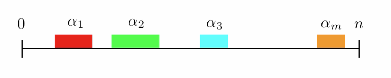
\includegraphics[width=0.4\linewidth]{imgs/def2_10.png}
    \caption{Markov subchains.}
    \label{fig:my_label}
\end{figure}

%%%%%%%%%%%%
\newpage
\subsection{Shannon's Information Measures}
- Entropy\\
- Conditional entropy\\
- Mutual information\\
- Conditional mutual information\\

\begin{tcolorbox}
\paragraph{Definition 2.13 (Entropy.)} The entropy $H(X)$ of a random variable $X$ is defined as
$$
H(X)=-\sum_{x} p(x) \log p(x)
$$
\begin{itemize}
    \item Convention: summation is taken over $\mathcal{S}_{X}$. 
    \item When the base of the logarithm is $\alpha,$ write $H(X)$ as $H_{\alpha}(X)$.
    \item Entropy measures the uncertainty of a discrete random variable.
    \item The unit for entropy is
        $$
        \begin{array}{ll}
        \text { bit } & \text { if } \alpha=2\\
        \text { nat } & \text { if } \alpha=e\\
        D-\mathrm{it} & \text { if } \alpha=D
        \end{array}
        $$
\end{itemize}
\end{tcolorbox}

\begin{tcolorbox}
\paragraph{Example (Binary Entropy Function).}
For $0 \leq \gamma \leq 1$, define the binary entropy function
$$
h_{b}(\gamma)=-\gamma \log \gamma-(1-\gamma) \log (1-\gamma)
$$
\end{tcolorbox}

\begin{figure}[!h]
    \centering
    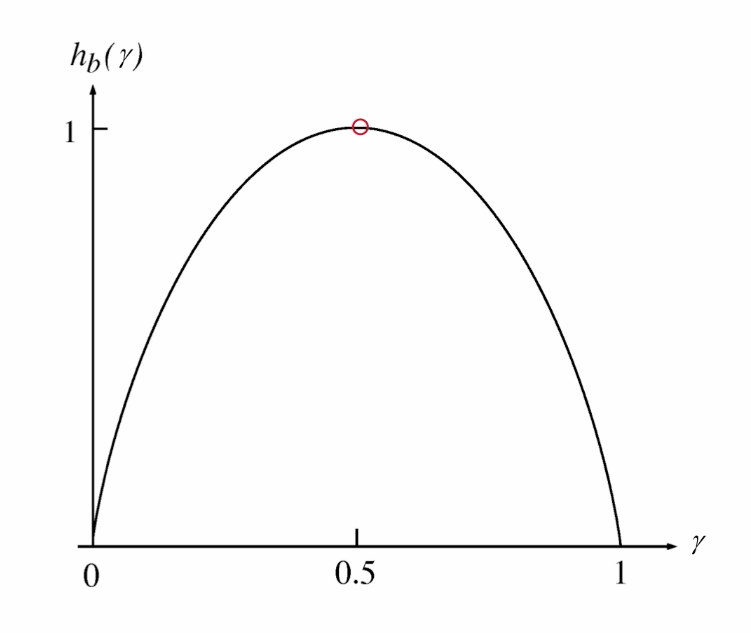
\includegraphics[width=0.3\linewidth]{imgs/exp2_13.png}
    \caption{Binary Entropy Function.}
    \label{fig:my_label}
\end{figure}

\begin{tcolorbox}
\paragraph{Definition 2.14 (Joint Entropy)} The joint entropy $H(X, Y)$ of a pair of random variables $X$ and $Y$ is defined as
$$
H(X, Y)=-\sum_{x, y} p(x, y) \log p(x, y)=-E \log p(X, Y)
$$
\paragraph{Definition 2.15 (Conditional Entropy)} For random variables $X$ and $Y,$ the conditional entropy of Ygiven $X$ is defined as
$$
H(Y \mid X)=-\sum_{x, y} p(x, y) \log p(y \mid x)=-E \log p(Y \mid X)
$$

\paragraph{Proposition 2.16}
$$
H(X, Y)=H(X)+H(Y \mid X)
$$
$$
H(X, Y)=H(Y)+H(X \mid Y)
$$
\end{tcolorbox}

\begin{tcolorbox}
\paragraph{Definition 2.17 (Mutual Information)} For random variables $X$ and $Y$, the mutual information between $X$ and $Y$ is defined as
$$
I(X ; Y)=\sum_{x, y} p(x, y) \log \frac{p(x, y)}{p(x) p(y)}=E \log \frac{p(X, Y)}{p(X) p(Y)}
$$
\paragraph{Remark} $I(X ; Y)$ is symmetrical in $X$ and $Y$.
\paragraph{Remark} Alternatively, we can write
$$
I(X ; Y)=\sum_{x, y} p(x, y) \log \frac{p(x, y)}{p(x) p(y)}=\sum_{x, y} p(x, y) \log \frac{p(x \mid y)}{p(x)}=E \log \frac{p(X \mid Y)}{p(X)}
$$
\paragraph{Proposition 2.18} The mutual information between a random variable $X$ and itself is equal to the entropy of $X,$ i.e., $I(X ; X)=H(X)$
\\
\paragraph{Proposition 2.19}
$$
\begin{aligned}
I(X ; Y) &=H(X)-H(X \mid Y) \\
I(X ; Y) &=H(Y)-H(Y \mid X)
\end{aligned}
$$
and
$$
I(X ; Y)=H(X)+H(Y)-H(X, Y)
$$
\end{tcolorbox}

\begin{figure}[!h]
    \centering
    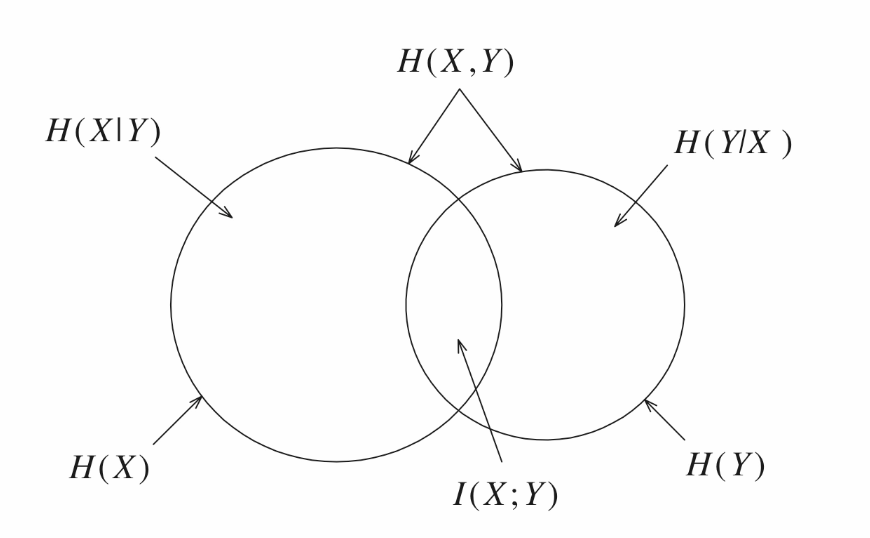
\includegraphics[width=0.5\linewidth]{imgs/def2_14.png}
    \caption{Information Diagram.}
    \label{fig:my_label}
\end{figure}

\begin{tcolorbox}
\paragraph{Definition 2.20} For random variables $X, Y$ and $Z,$ the mutual information between $X$ and $Y$ conditioning on $Z$ is defined as
$$
I(X ; Y \mid Z)=\sum_{x, y, z} p(x, y, z) \log \frac{p(x, y \mid z)}{p(x \mid z) p(y \mid z)}=E \log \frac{p(X, Y \mid Z)}{p(X \mid Z) p(Y \mid Z)}
$$
\end{tcolorbox}

\newpage
\subsection{Continuity of Shannon's Information Measures for Fixed Finite Alphabets}
\begin{tcolorbox}
\paragraph{Definition 2.23 (Variational Distance)} Let $p$ and $q$ be two probability distributions on a common alphabet $\mathcal{X}$. 'l'he variational distance between $p$ ind $q$ is defined as
$$
V(p, q)=\sum_{x \in \mathcal{X}^{\prime}} p(x)-q(x) \mid
$$
The entropy funetion is continuous at $p$ if
$$
\lim _{p^{\prime} \rightarrow p} H\left(p^{\prime}\right)-H\left(\lim _{p^{\prime} \rightarrow p^{\prime}} p^{\prime}\right)-H(p)
$$
or equivalently, for any $\epsilon>0,$ there exists $\delta \rightarrow 0$ such that
$$
\mid H(p)-H(q) \mid < \epsilon
$$
for all $q \in \mathcal{P}_{x}$ satisfying
$$
V(p, q)<\delta
$$
\end{tcolorbox}

\newpage
\subsection{Chain Rules}

\begin{tcolorbox}
\paragraph{Proposition 2.24(Chain Rule for Entropy)}
$$
H \left(X_{1}, X_{2}, \cdots, X_{n}\right)=\sum_{i=1}^{n} H\left(X_{i} \mid X_{1}, \cdots, X_{i-1}\right)
$$

\paragraph{Proposition 2.25 (Chain Rule for Conditional Entropy)}
$$
H\left(X_{1}, X_{2}, \cdots, X_{n} \mid Y\right)=\sum_{i=1}^{n} H\left(X_{i} \mid X_{1}, \cdots, X_{i-1}, Y\right)
$$

\paragraph{Proposition 2.26 (Chain Rule for Mutual Information)}
$$
I\left(X_{1}, X_{2}, \cdots, X_{n} ; Y\right)=\sum_{i=1}^{n} I\left(X_{i} ; Y \mid X_{1}, \cdots, X_{i-1}\right)
$$

\paragraph{Proposition 2.27 (Chain Rule for Conditional Mutual Information)}
$$
I\left(X_{1}, X_{2}, \cdots, X_{n} ; Y \mid Z\right)=\sum_{i=1}^{n} I\left(X_{i} ; Y \mid X_{1}, \cdots, X_{i-1}, Z\right)
$$
\end{tcolorbox}

\paragraph{Alternative Proof of Proposition 2.25}
$$
\begin{aligned}
H\left(X_{1}, X_{2}, \cdots, X_{n} \mid Y\right) &= \sum_{y} p(y) H\left(X_{1}, X_{2}, \cdots, X_{n} \mid Y=y\right) \\
&=\sum_{y} p(y) \sum_{i=1}^{n} H\left(X_{i} \mid X_{1}, \cdots, X_{i-1}, Y=y\right) \\
&=\sum_{i=1}^{n} \sum_{y} p(y) H\left(X_{i} \mid X_{1}, \cdots, X_{i-1}, Y=y\right) \\
&=\sum_{i=1}^{n} H\left(X_{i} \mid X_{1}, \cdots, X_{i-1}, Y\right)
\end{aligned}
$$
\paragraph{Remark} This alternative proof explains why Proposition 2.25 can be obtained from Proposition 2.24 by conditioning on $Y$.

\newpage
\subsection{Information Divergence}
\begin{tcolorbox}
\paragraph{Definition 2.28 (Information Divergence)} The informational divergence between two probability distributions $p$ and $q$ on a common alphabet $\mathcal{X}$ is defined as
$$
D(p \| q)=\sum_{x} p(x) \log \frac{p(x)}{q(x)}=E_{p} \log \frac{p(X)}{q(X)}
$$
where $E_{p}$ denotes expectation with respect to $p$

\paragraph{Convention:}
\begin{itemize}
    \item Summation is over $\mathcal{S}_{p},$ i.e., $\sum_{x \in \mathcal{S}_{p}}$
    \item $\operatorname{clog} \frac{c}{0}=\infty$ for $c>0$
    \item If $D(p \| q)<\infty,$ then $p(x)>0 \Rightarrow q(x)>0,$ or $\mathcal{S}_{p} \subset \mathcal{S}_{q}$
    \item $D(p \| q)$ measures the "distance" between $p$ and $q$
    \item $\boldsymbol{D}(p \| q)$ is not symmetrical in $p$ and $q,$ so $D(\cdot \| \cdot)$ is not a true metric.
    \item $D(\cdot \| \cdot)$ does not satisfy the triangular inequality. 
\end{itemize}
\end{tcolorbox}

\begin{tcolorbox}
\paragraph{Lemma 2.29 (Fundamental Inequality)} For any $a>0$,
$$
\ln a \leq a-1
$$
with equality if and only if $a=1$\\

\paragraph{Corollary 2.30} For any $a>0,$
$$
\ln a \geq 1-\frac{1}{a}
$$
with equality if and only if $a=1$.

\end{tcolorbox}
\begin{figure}[!h]
    \centering
    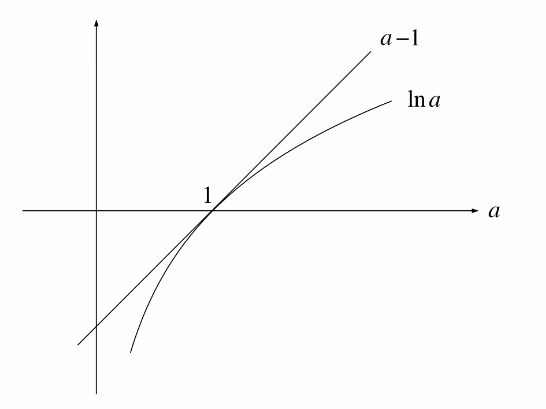
\includegraphics[width=0.5\linewidth]{imgs/def2_29.png}
    \caption{Information Diagram.}
    \label{fig:my_label}
\end{figure}

\begin{tcolorbox}
\paragraph{Theorem 2.31 (Divergence Inequality)} For any two probability distributions $p$ and $q$ on a common alphabet $\mathcal{X}$
$$
D(p \| q) \geq 0
$$
with equality if and only if $p=q$
\end{tcolorbox}
\paragraph{Proof.} For simplicity, assume $\mathcal{S}_{p}=\mathcal{S}_{\boldsymbol{q}}$, consider
$$
\begin{aligned}
D(p \| q) &=\sum_{x \in S_{p}} p(x) \log \frac{p(x)}{q(x)} \\
&=(\log c) \sum_{x \in \mathcal{S}_{p}} p(x) \ln \frac{p(x)}{q(x)} \\
& \geq(\log e) \sum_{x \in \mathcal{S}_{p}} p(x)\left(1-\frac{q(x)}{p(x)}\right) \\
&=(\log c)\left[\sum_{x \in \mathcal{S}_{p}} p(x)-\sum_{x \in \mathcal{S}_{p}} q(x)\right] \\
&=(\log e)\left[\sum_{x \in \mathcal{S}_{p}} p(x)-\sum_{x \in \mathcal{S}_{q}} q(x)\right] \\
&=0 .
\end{aligned}
$$
For equality to hold, further require
$$
\frac{p(x)}{q(x)}=1 \text { or } p(x)=q(x) \quad \text { for all } x \in \mathcal{S}_{p}
$$

\begin{tcolorbox}
\paragraph{Theorem 2.32 (Log-Sum Inequality)} For positive numbers $a_{1}, a_{2}, \cdots$ and nonnegative numbers $b_{1}, b_{2}, \cdots$ such that $\sum_{i} a_{i}<\infty$ and $0<\sum_{i} b_{i}<\infty$
$$
\sum_{i} a_{i} \log \frac{a_{i}}{b_{i}} \geq\left(\sum_{i} a_{i}\right) \log \frac{\sum_{i} a_{i}}{\sum_{i} b_{i}}
$$
with the convention that $\log \frac{a_{i}}{0}=\infty .$ Moreover, equality holds if and only if $\frac{a_{i}}{b_{i}}=$constant for all $i$
\\
\paragraph{Example:}
$$
a_{1} \log \frac{a_{1}}{b_{1}}+a_{2} \log \frac{a_{2}}{b_{2}} \geq\left(a_{1}+a_{2}\right) \log \frac{a_{1}+a_{2}}{b_{1}+b_{2}}
$$
\end{tcolorbox}
\paragraph{Proof.}
Let $a_{i}^{\prime}=a_{i} / \sum_{j} a_{j}$ and $b_{i}^{\prime}=b_{i} / \sum_{j} b_{j}$. Using the divergence inequality, we have
$$
\begin{aligned}
0 \leq & \sum_{i} a_{i}^{\prime} \log \frac{a_{i}^{\prime}}{b_{i}^{\prime}} \\
=& \sum_{i} \frac{a_{i}}{\sum_{j} a_{j}} \log \frac{a_{i} / \sum_{j} a_{j}}{b_{i} / \sum_{j} b_{j}} \\
=& \frac{1}{\sum_{j} a_{j}}\left[\sum_{i} a_{i} \log \frac{a_{i} / \sum_{j} a_{j}}{b_{i} / \sum_{j} b_{j}}\right] \\
=& \frac{1}{\sum_{j} a_{j}}\left[\sum_{i} a_{i} \log \frac{a_{i}}{b_{i}}-\sum_{i} a_{i} \log \frac{\sum_{j} a_{j}}{\sum_{j} b_{j}}\right] \\
=& \frac{1}{\sum_{j} a_{j}}\left[\sum_{i} a_{i} \log \frac{a_{i}}{b_{i}}-\left(\sum_{i} a_{i}\right) \log \frac{\sum_{j} a_{j}}{\sum_{j} b_{j}}\right]
\end{aligned}
$$

\paragraph{Remark} Divergence Inequality vs Log-Sum Inequality are equivalent.


\begin{tcolorbox}
\paragraph{Theorem 2.33 (Pinsker's Inequality)}
$$
D(p \| q) \geq \frac{1}{2 \ln 2} V^{2}(p, q)
$$
\begin{itemize}
    \item If $D(p \| q)$ or $D(q \| p)$ is small, then so is $V(p, q)=V(q, p)$
    \item For a sequence of probability distributions $q_{k},$ as $k \rightarrow \infty,$ if $D\left(p \| q_{k}\right) \rightarrow 0$ $\operatorname{or} D\left(q_{k} \| p\right) \rightarrow 0,$ then $V\left(p, q_{k}\right)=V\left(q_{k}, p\right) \rightarrow 0$
    \item That is, "convergence in divergence" is a stronger notion than "convergence in variational distance."
\end{itemize}
\end{tcolorbox}

\newpage
\subsection{Basic Inequalities}
\begin{tcolorbox}
\paragraph{Theorem 2.34} For random variables $X, Y,$ and $Z,$
$$
I(X ; Y \mid Z) \geq 0
$$
with equality if and only if $X$ and $Y$ are independent when conditioning on $Z$.
\\
\paragraph{Corollary} All Shannon's information measures are nonnegative, because they are all special cases of conditional mutual information.

\end{tcolorbox}
\paragraph{Proof}
$$
\begin{aligned}
I(X ; Y \mid Z) = & \sum_{x, y, z} p(x, y, z) \log \frac{p(x, y \mid z)}{p(x \mid z) p(y \mid z)} \\
= & \sum_{z} \sum_{x, y} p(x, y, z) \log \frac{p(x, y \mid z)}{p(x \mid z) p(y \mid z)} \\
= & \sum_{z} \sum_{x, y} p(z) p(x, y \mid z) \log \frac{p(x, y \mid z)}{p(x \mid z) p(y \mid z)} \\
= & \sum_{z} p(z) \sum_{x, y} p(x, y \mid z) \log \frac{p(x, y \mid z)}{p(x \mid z) p(y \mid z)} \\
= & \sum_{z} p(z) D\left(p_{X Y \mid z} \| p_{X \mid z} p_{Y \mid z}\right)
\end{aligned}
$$

\begin{tcolorbox}
\paragraph{Proposition 2.35} $ H(X)=0$ if and only if $X$ is deterministic.\\
\paragraph{Proposition 2.36} $H(Y \mid X)=0$ if and only if $Y$ is a function of $X$
$$
H(Y \mid X)=\sum_{x} p(x) H(Y \mid X=x)
$$

\paragraph{Proposition 2.37} $I(X ; Y)=0$ if and only if $X$ and $Y$ are independent.\\
\end{tcolorbox}

\newpage
\subsection{Some Useful Information Inequalities}
\begin{tcolorbox}
\paragraph{Theorem 2.38 (Conditioning Does Not Increase Entropy)}
$$
H(Y \mid X) \leq H(Y)
$$
with equality if and only if $X$ and $Y$ are independent.
\\
\paragraph{Proof}
$$
H(Y \mid X)=H(Y)-I(X ; Y) \leq H(Y)
$$
with equality if and only if $I(X ; Y)=0,$ or $X$ and $Y$ are independent.
\\

\begin{itemize}
    \item Similarly, $H(Y \mid X, Z) \leq H(Y \mid Z)$
    \item Warning: \textcolor{blue}{$I(X ; Y \mid Z) \leq I(X ; Y)$ does not hold in general.}
\end{itemize}
\end{tcolorbox}

\begin{tcolorbox}
\paragraph{Theorem 2.39 (Independence Bound for Entropy)}
$$
H\left(X_{1}, X_{2}, \cdots, X_{n}\right) \leq \sum_{i=1}^{n} H\left(X_{i}\right)
$$
with equality if and only if $X_{i}, i=1,2, \cdots, n$ are mutually independent.
\end{tcolorbox}
\paragraph{Proof} By the chain rule for entropy,
$$
\begin{aligned}
H\left(X_{1}, X_{2}, \cdots, X_{n}\right)
=&\sum_{i=1}^{n} H\left(X_{i} \mid X_{1}, \ldots, X_{i-1}\right) \\
\leq& \sum_{i=1}^{n} H\left(X_{i}\right)
\end{aligned}
$$
The inequality is tight iff it is tight for each $i$, i.e., 
$H\left(X_{i} \mid X_{1}, \cdots, X_{i-1}\right)=H\left(X_{i}\right)$

$$
\begin{aligned}
p\left(x_{1}, x_{2}, \cdots, x_{n}\right) 
=& p\left(x_{1}, x_{2}, \cdots, x_{n-1}\right) p\left(x_{n}\right) \\
=& p\left(x_{1}, x_{2}, \cdots, x_{n-2}\right) p\left(x_{n-1}\right) p\left(x_{n}\right) \\
=& p\left(x_{1}\right) p\left(x_{2}\right) \cdot \cdots p\left(x_{n}\right)
\end{aligned}
$$

\begin{tcolorbox}
\paragraph{Theorem 2.40}
$$
I(X ; Y, Z) \geq I(X ; Y)
$$
with equality if and only if $X \rightarrow Y \rightarrow Z$ forms a Markov chain.
\end{tcolorbox}

\paragraph{Proof} By the chain rule for mutual information, we have
$$
I(X ; Y, Z)=I(X ; Y)+I(X ; Z \mid Y) \geq I(X ; Y)
$$
The above inequality is tight iff $I(X ; Z \mid Y) = 0$ (or $X \rightarrow Y \rightarrow Z$ forms a Markov chain.)

\begin{tcolorbox}
\paragraph{Lemma 2.41} If $X \rightarrow Y \rightarrow Z$ forms a Markov chain, then
$$
I(X ; Z) \leq I(X ; Y)
$$
$$
I(X ; Z) \leq I(Y ; Z)
$$

\paragraph{Corollary} If $X \rightarrow Y \rightarrow Z,$ then 
$$
H(X \mid Z) \geq H(X \mid Y)
$$
\end{tcolorbox}

\paragraph{Proof Corollary}
$1 .$ Assume $X \rightarrow Y \rightarrow Z,$ i.e., $X \perp Z \mid Y$. Then
$$
I(X ; Z \mid Y)=0
$$
2. Consider
\textcolor{blue}{
$$
\begin{aligned}
I(X ; Z) & \stackrel{a}{=} I(X ; Y, Z)-I(X ; Y \mid Z) \\
& \leq I(X ; Y, Z) \\
& \stackrel{b}{=} I(X ; Y)+I(X ; Z \mid Y) \\
&=I(X ; Y)
\end{aligned}
$$
}
a) Chain rule for mutual information:
\textcolor{blue}{
$$
\begin{aligned}
& I(X ; Y, Z)=I(X ; Z)+I(X ; Y \mid Z) \\
\Rightarrow \quad & I(X ; Z)=I(X ; Y, Z)-I(X ; Y \mid Z)
\end{aligned}
$$
}
b) Chain rule for mutual information \\
3. since $X \rightarrow Y \rightarrow Z$ is equivalent to $Z \rightarrow Y \rightarrow X$
we also have proved (2) by symmetry.

\paragraph{Proof}
$$
\begin{aligned}
H(X \mid Z) &=H(X)-I(X ; Z) \\
& \geq H(X)-I(X ; Y) \\
&=H(X \mid Y)
\end{aligned}
$$
\paragraph{Remark} Suppose $Y$ is an observation of $X$. Then further processing of $Y$ can only increase the uncertainty about $X$ on the average.

\begin{tcolorbox}
\paragraph{Theorem 2.42 (\textcolor{blue}{Data Processing Theorem})} If $U \rightarrow X \rightarrow Y \rightarrow V$ forms a Markov chain, then
$$
I(U ; V) \leq I(X ; Y)
$$
\end{tcolorbox}
\paragraph{Proof} For two subchains
$$
\begin{array}{l}
U \rightarrow X \rightarrow Y \\
U \rightarrow Y \rightarrow V
\end{array}
$$
By applying Lemma 2.41
$$
I(U ; V) \leq I(U ; Y) \leq I(X ; Y)
$$

\newpage
\subsection{Fano's Inequality}
\begin{tcolorbox}
\paragraph{Theorem 2.43} For any random variable $X$,
$$
H(X) \leq \log |\mathcal{X}|
$$
where $|\mathcal{X}|$ denotes the size of the alphabet $\mathcal{X}$. This upper bound is tight if and only if $X$ is distributed uniformly on $\mathcal{X}$.
\end{tcolorbox}

\paragraph{Remark} For a random variable $X,$ if the alphabet is finite, then
$$
H(X) \leq \log |\mathcal{X}|<\infty
$$
i.e., $H(X)$ is finite.

\paragraph{Proof} Let $u$ be the uniform distribution on $\mathcal{X},$ i.e.,
$$
u(x)=\frac{1}{|\mathcal{X}|} \quad \text { for all } x \in \mathcal{X}
$$
Then
$$
\begin{aligned}
\log |\mathcal{X}|-H(X) =&-\sum_{x \in \mathcal{S}_{X}} p(x) \log \frac{1}{|\mathcal{X}|}+\sum_{x \in \mathcal{S}_{X}} p(x) \log p(x) \\
=&-\sum_{x \in \mathcal{S}_{X}} p(x) \log u(x)+\sum_{x \in \mathcal{S}_{X}} p(x) \log p(x) \\
=& \sum_{x \in \mathcal{S}_{X}} p(x) \log \frac{p(x)}{u(x)} \\
=& D(p \| u) \geq 0
\end{aligned}
$$

\begin{tcolorbox}
\paragraph{Theorem 2.47 (Fano's Inequality)} Let $X$ and $\hat{X}$ be random variables taking values in the same alphabet $\mathcal{X}$. Then
$$
H(X \mid \hat{X}) \leq h_{b}\left(P_{e}\right)+P_{e} \log (|\mathcal{X}|-1)
$$
where $P_{e}=\operatorname{Pr}\{X \neq \hat{X}\}$ and $h_{b}$ is the binary entropy function.
\\
\paragraph{Corollary 2.48}
$H(X \mid \hat{X})< 1 +P_{e} \log |\mathcal{X}|$
\end{tcolorbox}

\subsection{Entropy Rate of a Stationary Source}
\paragraph{Definition 2.54} The entropy rate of an information source $\left\{X_{k}\right\}$ is defined as
$$
H_{X}=\lim _{n \rightarrow \infty} \frac{1}{n} H\left(X_{1}, X_{2}, \cdots, X_{n}\right)
$$
when the limit exists.


\newpage
\section{The I-Measure}
$$
\begin{aligned}
H / I \quad & \quad \leftrightarrow \mu^{*} \\
, \quad & \quad \leftrightarrow \cup \\
; \quad & \quad \leftrightarrow  \cap \\
\mid \quad & \quad \leftrightarrow -\left(A-B=A \cap B^{c}\right)
\end{aligned}
$$

\paragraph{1. Examples}
$$
\begin{aligned}
H\left(X_{1} \mid X_{2}\right) &=\mu^{*}\left(\tilde{X}_{1}-\tilde{X}_{2}\right) \\
H\left(X_{2} \mid X_{1}\right) &=\mu^{*}\left(\tilde{X}_{2}-\tilde{X}_{1}\right) \\
I\left(X_{1} ; X_{2}\right) &=\mu^{*}\left(\bar{X}_{1} \cap \tilde{X}_{2}\right)
\end{aligned}
$$

\paragraph{2. Inclusion-Exclusion formulation in set-theory}
$$
\mu^{*}\left(\tilde{X}_{1} \cup \tilde{X}_{2}\right)=\mu^{*}\left(\tilde{X}_{1}\right)+\mu^{*}\left(\tilde{X}_{2}\right)-\mu^{*}\left(\tilde{X}_{1} \cap \tilde{X}_{2}\right)
$$
corresponds to
$$
H\left(X_{1}, X_{2}\right)=H\left(X_{1}\right)+H\left(X_{2}\right)-I\left(X_{1} ; X_{2}\right)
$$
in information theory.

\subsection{Preliminaries}
\paragraph{Definition 3.1} The field $\mathcal{F}_{n}$ generated by sets $\tilde{X}_{1}, \tilde{X}_{2}, \cdots, \tilde{X}_{n}$ is the collection of sets which can be obtained by any sequence of usual set operations (union, intersection, complement, and difference) on $\tilde{X}_{1}, \tilde{X}_{2}, \cdots, \tilde{X}_{n}$

\paragraph{Definition 3.2} The atoms of $\mathcal{F}_{n}$ are sets of the form $\cap_{i=1}^{n} Y_{i},$ where $Y_{i}$ is either $\bar{X}_{i}$ or $\bar{X}_{i}^{c},$ the complement of $\bar{X}_{i}$

\paragraph{Example 3.3}
\begin{itemize}
    \item The sets $\tilde{X}_{1}$ and $\tilde{X}_{2}$ generate the field $\mathcal{F}_{2}$
    \item There are 4 atoms in $\mathcal{F}_{2}$ :
        $$
        \tilde{X}_{1} \cap \tilde{X}_{2},\quad \tilde{X}_{1}^{c} \cap \tilde{X}_{2},\quad \tilde{X}_{1} \cap \tilde{X}_{2}^{c}, \quad \tilde{X}_{1}^{c} \cap \tilde{X}_{2}^{c}
        $$
    \item There are a total of $2^{4}=16$ sets in $\mathcal{F}_{2},$ formed by the unions of the above 4 atoms.
\end{itemize}

\paragraph{Definition 3.4} A real function $\mu$ defined on $\mathcal{F}_{n}$ is called a signed measure if it is set-additive, i.e., for disjoint $A$ and $B$ in $\mathcal{F}_{n}$
$$
\mu(A \cup B)=\mu(A)+\mu(B)
$$
Remark: A signed measure can take positive or negative values. If a signed measure takes only positive values, it is simply called a measure.

\newpage
\subsection{Construction of the I-Measure $\mu^{*}$}
\begin{tcolorbox}
\paragraph{Notations} 
For nonempty subset $G$ of $\mathcal{N}_{n}$ :
$\boldsymbol{X}_{G}=\left(X_{i}, i \in G\right)$ \qquad
$\boldsymbol{\tilde { X }}_{G}=\cup_{i \in G} \tilde{X}_{i}$
\\
\paragraph{Theorem 3.6} Let
$$
\mathcal{B}=\left\{\tilde{X}_{G}: G \text { is a nonempty subset of } \mathcal{N}_{n}\right\}
$$
Then a signed measure $\mu$ on $\mathcal{F}_{n}$ is completely specified by $\{\mu(B), B \in \mathcal{B}\},$ which can be any set of real numbers.

\paragraph{Remark} We have seen that a signed measure $\mu$ on $\mathcal{F}_{n}$ is completely specified by $\{\mu(A), A \in \mathcal{A}\},$ the set of values of $\mu$ on the nonempty atoms. This theorem says that $\mu$ can instead be specified by $\{\mu(B), B \in \mathcal{B}\}$, the set of values of $\mu$ on the unions.
\end{tcolorbox}

\begin{tcolorbox}
\paragraph{The Inclusion-Exclusion Formula}
$$
\begin{aligned}
\mu\left(\bigcup_{k=1}^{m} A_{k}\right)=& \sum_{1 \leq i \leq m} \mu\left(A_{i}\right)-\sum_{1 \leq i<j \leq m} \mu\left(A_{i} \cap A_{j}\right)+\cdots \\
&+(-1)^{m+1} \mu\left(A_{1} \cap A_{2} \cap \cdots \cap A_{m}\right)
\end{aligned}
$$

\paragraph{Theorem 3.19 (Variation of the Inclusion-Exclusion Formula)}
$$
\begin{aligned}
\mu\left(\bigcap_{k=1}^{m} A_{k}-B\right)=& \sum_{1 \leq i \leq m} \mu\left(A_{i}-B\right)-\sum_{1 \leq i<j \leq m} \mu\left(A_{i} \cup A_{j}-B\right)+\cdots \\
&+(-1)^{m+1} \mu\left(A_{1} \cup A_{2} \cup \cdots \cup A_{m}-B\right)
\end{aligned}
$$
\end{tcolorbox}
\begin{tcolorbox}
\paragraph{Proof of Lemma 3.7}
$$
\begin{aligned}
\mu(A \cap B-C)=& \mu(A-C)+\mu(B-C)-\mu(A \cup B-C) \\
=&(\mu(A \cup C)-\mu(C))+(\mu(B \cup C)-\mu(C)) -(\mu(A \cup B \cup C)-\mu(C)) \\
=& \mu(A \cup C)+\mu(B \cup C)-\mu(A \cup B \cup C)-\mu(C)
\end{aligned}
$$
\paragraph{Proof of Lemma 3.8}
$$
\begin{aligned}
I(X ; Y \mid Z) &=H(X \mid Z)-H(X \mid Y, Z) \\
&=H(X, Z)-H(Z)-(H(X, Y, Z)-H(Y, Z)) \\
&=H(X, Z)+H(Y, Z)-H(X, Y, Z)-H(Z)
\end{aligned}
$$
\end{tcolorbox}

\begin{tcolorbox}
\paragraph{Construction of the $I$ -Measure $\mu^{*}$ on $\mathcal{F}_{n}$}
Define $\mu^{*}$ by setting
$$
\mu^{*}\left(\tilde{X}_{G}\right)=H\left(X_{G}\right)
$$
for all nonempty subsets $G$ of $\mathcal{N}_{n}$
- That is, the value of $\mu^{*}$ on the union of a collection $G$ of set variables is equal to the joint entropy of the collection $G$ of random variables.
\end{tcolorbox}
\begin{tcolorbox}
\paragraph{Theorem 3.9} $\mu^{*}$ is the unique signed measure on $\mathcal{F}_{n}$ which is consistent with all Shannon's information measures.
\\
\paragraph{Implications}
Can formally regard Shannon's information measures for $n$ r.v.'s as the unique signed measure $\mu^{*}$ defined on $\mathcal{F}_{n}$
Can employ set-theoretic tools to manipulate expressions of Shannon's information measures.
\end{tcolorbox}

\newpage
\subsection{$\mu^{*}$ can be Negative}
For $n=3,$ the values of $\mu^{*}$ on the nonempty atoms of $\mathcal{F}_{3}$ all correspond to Shannon's information measures, except
$$
\mu^{*}\left(\tilde{X}_{1} \cap \tilde{X}_{2} \cap \tilde{X}_{3}\right)=I\left(X_{1} ; X_{2} ; X_{3}\right)
$$
We will show that it is possible to construct r.v.'s $X_{1}, X_{2},$ and $X_{3}$ such that $\mu^{*}\left(\tilde{X}_{1} \cap \tilde{X}_{2} \cap \tilde{X}_{3}\right)<0$

\paragraph{Example 3.10} 
Let $X_{1}$ and $X_{2}$ be independent binary random variables with uniform distribution, i.e.,
$$
\operatorname{Pr}\left\{X_{i}=0\right\}=\operatorname{Pr}\left\{X_{i}=1\right\}=0.5, \qquad i=1,2
$$
Let
\textcolor{blue}{
$$
X_{3}=\left(X_{1}+X_{2}\right) \bmod 2
$$
}
It is easy to check that $X_{3}$ also has a uniform distribution. Thus,
$H\left(X_{i}\right)=1$ for $i=1,2,3$.\\
It is also easy to check that $X_{1}, X_{2},$ and $X_{3}$ are pairwise independent. Therefore,
$$
H\left(X_{i}, X_{j}\right)=2
\qquad
I\left(X_{i} ; X_{j}\right)=0
$$
for $1 \leq i<j \leq 3$
We see from (1) that $X_{3}$ is a function of $X_{1}$ and $X_{2},$ so that
$$
H\left(X_{3} \mid X_{1}, X_{2}\right)=0
$$
Then by the chain rule for entropy, we have
$$
H\left(X_{1}, X_{2}, X_{3}\right) = H\left(X_{1}, X_{2}\right)+H\left(X_{3} \mid X_{1}, X_{2}\right)
= 2+0 = 2
$$
Now for distinct $1 \leq i, j, k \leq 3$
$$
\begin{aligned}
I\left(X_{i} ; X_{j} \mid X_{k}\right)
=& H\left(X_{i}, X_{k}\right)+H\left(X_{j}, X_{k}\right) -H\left(X_{1}, X_{2}, X_{3}\right)-H\left(X_{k}\right) \\
=&2+2-2-1 = 1
\end{aligned}
$$
It then follows that
\textcolor{blue}{
$$
\begin{aligned}
\mu^{*} \left(\tilde{X}_{1} \cap \bar{X}_{2} \cap \tilde{X}_{3}\right) &=\mu^{*}\left(\bar{X}_{1} \cap \bar{X}_{2}\right)-\mu^{*}\left(\bar{X}_{1} \cap \tilde{X}_{2}-\bar{X}_{3}\right) \\
&= I\left(X_{1} ; X_{2}\right)-I\left(X_{1} ; X_{2} \mid X_{3}\right) \\
&=0-1 <0
\end{aligned}
$$
}
\begin{figure}[!h]
    \centering
    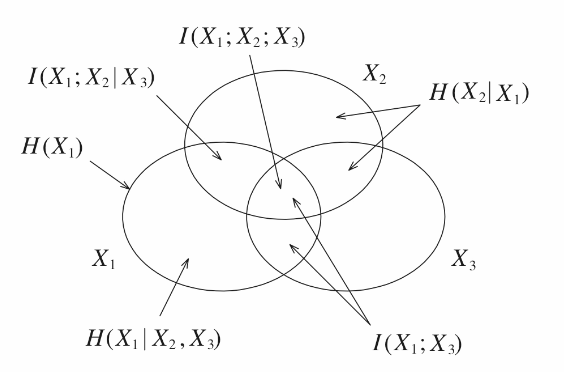
\includegraphics[width=0.33\linewidth]{imgs/exp3_10.png}
    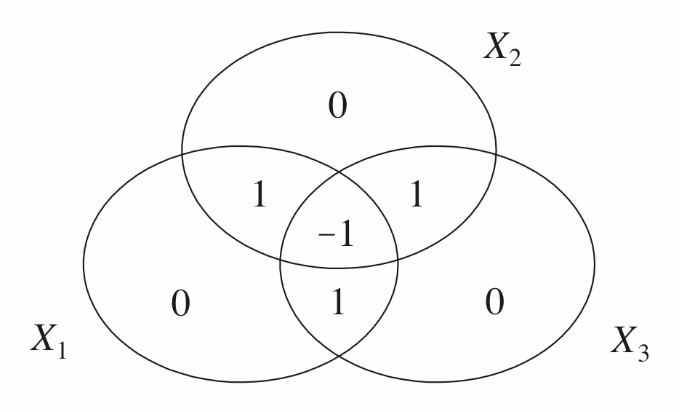
\includegraphics[width=0.3\linewidth]{imgs/exp3_10_2.png}
    \caption{$\mu^{*}$ can be Negative.}
    \label{fig:my_label}
\end{figure}

\begin{tcolorbox}
\paragraph{Theorem 3.11} If there is no constraint on $X_{1}, X_{2}, \cdots, X_{n},$ then $\mu^{*}$ can take any set of nonnegative values on the nonempty atoms of $\mathcal{F}_{n}$. 
\end{tcolorbox}
Evidently, we can take $\mu^{*}(A)=H\left(Y_{A}\right)$ for all $A \in \mathcal{A}$. By the uniqueness of $\mu^{*}$ (Theorem 3.9), this is also the only possibility for $\mu^{*}$


\newpage
\subsection{Information Diagrams for Markov Chains}
\begin{itemize}
    \item If $X_{1} \rightarrow X_{2} \rightarrow \cdots \rightarrow X_{n}$ form a Markov chain, then the structure of $\mu^{*}$ is much simpler and hence the information diagram can be simplified.
    \item For $n=3, X_{1} \rightarrow X_{2} \rightarrow X_{3}$ iff $I\left(X_{1} ; X_{3} \mid X_{2}\right)=0,$ or $\mu^{*}\left(\tilde{X}_{1} \cap \tilde{X}_{3}-\tilde{X}_{2}\right)=0$
    \item So the atom $\tilde{X}_{1} \cap \tilde{X}_{3}-\tilde{X}_{2}$ can be suppressed in the information diagram.
\end{itemize}
\begin{figure}[!h]
    \centering
    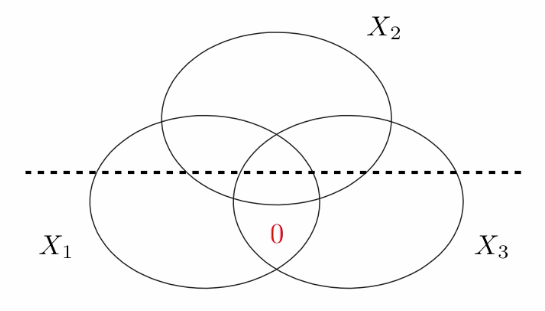
\includegraphics[width=0.33\linewidth]{imgs/exp3_4_1.png} \qquad
    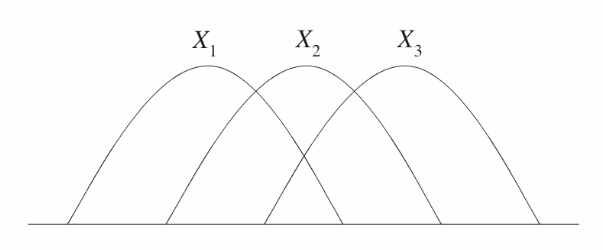
\includegraphics[width=0.4\linewidth]{imgs/exp3_4_2.png}
    \caption{Suppressed information diagram.}
    \label{fig:my_label}
\end{figure}

\paragraph{Illustration:} $\mu^{*}$ for $X_{1} \rightarrow X_{2} \rightarrow X_{3}$\\
In this information diagram,
$$
\begin{aligned}
I\left(X_{1} ; X_{3} \mid X_{2}\right) &=\mu^{*}\left(\tilde{X}_{1} \cap \tilde{X}_{3}-\tilde{X}_{2}\right) \\
&=\mu^{*}(\emptyset) \\
&=0
\end{aligned}
$$
Also,
$$
\begin{aligned}
\mu^{*}\left(\tilde{X}_{1} \cap \tilde{X}_{2} \cap \tilde{X}_{3}\right) &=\mu^{*}\left(\tilde{X}_{1} \cap \tilde{X}_{3}\right) \\
&=I\left(X_{1} ; X_{3}\right) \\
& \geq 0
\end{aligned}
$$
Since the values of $\mu^{*}$ on all the remaining atoms correspond to Shannon's information measures and hence are nonnegative, we conclude that $\mu^{*}$ is a measure.

\begin{figure}[!h]
    \centering
    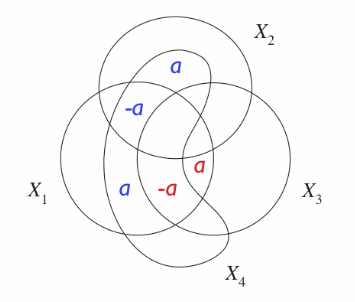
\includegraphics[width=0.28\linewidth]{imgs/exp3_4_5.png}
    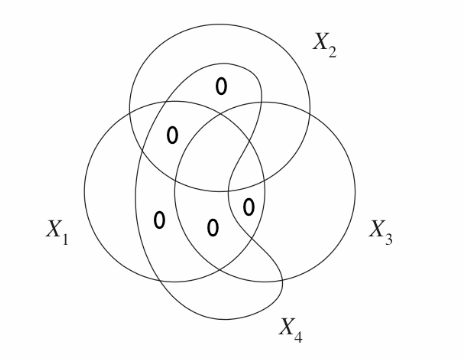
\includegraphics[width=0.3\linewidth]{imgs/exp3_4_3.png} \qquad
    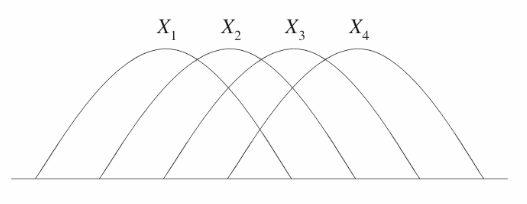
\includegraphics[width=0.35\linewidth]{imgs/exp3_4_4.png}
    \caption{Suppressed information diagram.}
    \label{fig:my_label}
\end{figure}
\paragraph{Illustration:} Structure of $\mu^{*}$ for $X_{1} \rightarrow X_{2} \rightarrow X_{3} \rightarrow X_{4}$
\\
1. The Markov subchain $X_{1} \rightarrow X_{2} \rightarrow X_{3}$ implies
$0=I\left(X_{1} ; X_{3} \mid X_{2}\right)=I\left(X_{1} ; X_{3} ; X_{4} \mid X_{2}\right)+I\left(X_{1} ; X_{3} \mid X_{2}, X_{4}\right)$
Let $I\left(X_{1} ; X_{3} \mid X_{2}, X_{4}\right)=a \geq 0 .$ Then
$$
I\left(X_{1} ; X_{3} ; X_{4} \mid X_{2}\right)=-a
$$
2. The Markov subchain $X_{1} \rightarrow X_{2} \rightarrow X_{4}$ implies
$0=I\left(X_{1} ; X_{4} \mid X_{2}\right)=I\left(X_{1} ; X_{3} ; X_{4} \mid X_{2}\right)+I\left(X_{1} ; X_{4} \mid X_{2}, X_{3}\right)$
since $I\left(X_{1} ; X_{3} ; X_{4} \mid X_{2}\right)=-a$
$$
I\left(X_{1} ; X_{4} \mid X_{2}, X_{3}\right)=a
$$
3. The Markov subchain $X_{1} \rightarrow X_{3} \rightarrow X_{4}$ implies
$0=I\left(X_{1} ; X_{4} \mid X_{3}\right)=I\left(X_{1} ; X_{2} ; X_{4} \mid X_{3}\right)+I\left(X_{1} ; X_{4} \mid X_{2}, X_{3}\right)$
since $I\left(X_{1} ; X_{4} \mid X_{2}, X_{3}\right)=a$
$$
I\left(X_{1} ; X_{2} ; X_{4} \mid X_{3}\right)=-a
$$
4. The Markov subchain $X_{2} \rightarrow X_{3} \rightarrow X_{4}$ implies
$0=I\left(X_{2} ; X_{4} \mid X_{3}\right)=I\left(X_{1} ; X_{2} ; X_{4} \mid X_{3}\right)+I\left(X_{2} ; X_{4} \mid X_{1}, X_{3}\right)$
$\sin \operatorname{ce} I\left(X_{1} ; X_{2} ; X_{4} \mid X_{3}\right)=-a$
$$
I\left(X_{2} ; X_{4} \mid X_{1}, X_{3}\right)=a
$$
5. The Markov subchain $\left(X_{1}, X_{2}\right) \rightarrow X_{3} \rightarrow X_{4}$ implies
$$
0=I\left(X_{1}, X_{2} ; X_{4} \mid X_{3}\right)=
I\left(X_{1} ; X_{4} \mid X_{2}, X_{3}\right)+I\left(X_{1} ; X_{2} ; X_{4} \mid X_{3}\right)+I\left(X_{2} ; X_{4} \mid X_{1}, X_{3}\right)
$$
Then
$$
0=a-a+a=a
$$
Therefore $a=0,$ and so $\mu^{*}$ vanishes on the corresponding 5 atoms as shown in the information diagram.

\newpage
\subsection{Examples of Applications}
\begin{tcolorbox}
\paragraph{Example 3.12 (Concavity of Entropy)} Let $X_{1} \sim p_{1}(x)$ and $X_{2} \sim p_{2}(x)$, and
$$
X \sim p(x)=\lambda p_{1}(x)+\bar{\lambda} p_{2}(x)
$$
where $0 \leq \lambda \leq 1$ and $\bar{\lambda}=1-\lambda$. Show that
$
H(X) \geq \lambda H\left(X_{1}\right)+\bar{\lambda} H\left(X_{2}\right)
$
\end{tcolorbox}
\paragraph{Proof.}
$$
\begin{aligned}
H(X) \geq & H(X \mid Z) \\
= & \operatorname{Pr}\{Z=1\} H(X \mid Z=1)+\operatorname{Pr}\{Z=2\} H(X \mid Z=2) \\
= & \lambda H\left(X_{1}\right)+\bar{\lambda} H\left(X_{2}\right)
\end{aligned}
$$
This shows that \textcolor{blue}{$H(X)$ is a concave functional of $p(x)$}

\paragraph{Interpretation} The entropy of a mixture of distributions is \textcolor{blue}{at least} the mixture of the corresponding entropies.

\begin{tcolorbox}
\paragraph{Example 3.13/3.14 (Convexity/Concavity of Mutual Information)} Let
$$
(X, Y) \sim p(x, y)=p(x) p(y \mid x)
$$
Show that for fixed \textcolor{blue}{$p(x), I(X ; Y)$ is a convex functional of $p(y \mid x)$}.\\
Show that for fixed \textcolor{blue}{$p(y \mid x), I(X ; Y)$ is a concave functional of $p(x)$}
\end{tcolorbox}
\paragraph{Proof 3.13}
$$
\begin{aligned}
I(X ; Y) =& I(X ; Y \mid Z)+I(X ; Y ; Z) \\
\leq & I(X ; Y \mid Z) \\
=& \operatorname{Pr}\{Z=1\} I(X ; Y \mid Z=1) +\operatorname{Pr}\{Z=2\} I(X ; Y \mid Z=2) \\
=& \lambda I\left(p(x), p_{1}(y \mid x)\right)+\bar{\lambda} I\left(p(x), p_{2}(y \mid x)\right)
\end{aligned}
$$
\paragraph{Interpretation} For a fixed input distribution $p(x)$, the mutual information between the input and the output of the system as shown, which is obtained by mixing 2 channels $p_{1}(y \mid x)$ and $p_{2}(y \mid x),$ is \textcolor{blue}{at most} the mixture of the 2 mutual informations corresponding to $p_{1}(y \mid x)$ and $p_{2}(y \mid x),$ respectively

\paragraph{Proof 3.14}
$$
\begin{aligned}
I(X ; Y)
\geq & I(X ; Y \mid Z) \\
=& \operatorname{Pr}\{Z=1\} I(X ; Y \mid Z=1) +\operatorname{Pr}\{Z=2\} I(X ; Y \mid Z=2) \\
=& \lambda I\left(p_{1}(x), p(y \mid x)\right)+\bar{\lambda} I\left(p_{2}(x), p(y \mid x)\right)
\end{aligned}
$$
This shows that for fixed $p(y \mid x), I(X ; Y)$ is a concave functional of $p(x)$

\paragraph{Interpretation} For a fixed channel, by mixing the input distribution, the mutual information is at least equal to the mixture of the corresponding mutual informations.

\begin{figure}[!h]
    \centering
    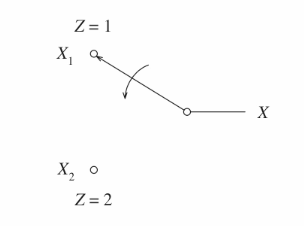
\includegraphics[width=0.22\linewidth]{imgs/exp3_12.png}
    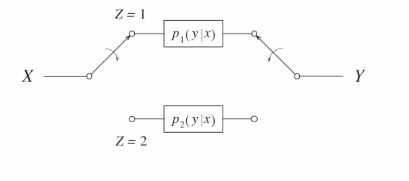
\includegraphics[width=0.3\linewidth]{imgs/exp3_13.png} \qquad
    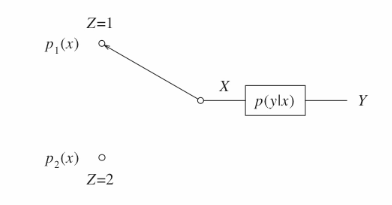
\includegraphics[width=0.3\linewidth]{imgs/exp3_14.png}
    \caption{Systems}
    \label{fig:my_label}
\end{figure}

\begin{tcolorbox}
\paragraph{Shannon's Perfect Secrecy Theorem}
\begin{itemize}
    \item Perfect Secrecy: $I(X ; Y)=0$
    \item Decipherability: $H(X \mid Y, Z)=0$
    \item These implies $H(Z) \geq H(X),$ i.e., the length of the key is at least the same as the length of the plaintext.
    \item Shannon (1949) gave a combinatorial proof. Can readily be proved by an information diagram.
\end{itemize}
\end{tcolorbox}

\begin{figure}[!t]
    \centering
    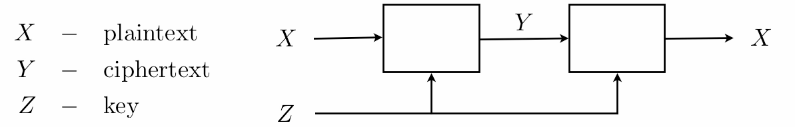
\includegraphics[width=0.5\linewidth]{imgs/exp3_15.png} \qquad
    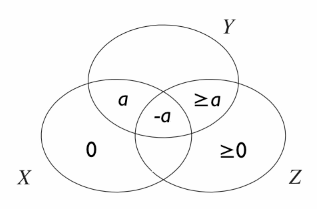
\includegraphics[width=0.2\linewidth]{imgs/exp3_15_2.png}
    \caption{Shannon's Perfect Secrecy Theorem}
    \label{fig:my_label}
\end{figure}


\paragraph{Example 3.15 (Imperfect Secrecy Theorem)} Let $X$ be the plain text, $Y$ be the cipher text, and $Z$ be the key in a secret key cryptosystem. since $X$ can be recovered from $Y$ and $Z,$ we have
$$
H(X \mid Y, Z)=0
$$
Show that this constraint implies
$$
I(X ; Y) \geq H(X)-H(Z)
$$

\paragraph{Remark}
$I(X ; Y)$ measures the "leakage of information." When $I(X ; Y)=0,$ it reduces Shannon's perfect secrecy theorem.

\begin{tcolorbox}
\paragraph{Example 3.17 (Data Processing Theorem)} If $X \rightarrow Y \rightarrow Z \rightarrow T$, then
\begin{itemize}
    \item $I(X ; T) \leq I(Y ; Z)$
    \item $I(Y ; Z)=I(X ; T)+I(X ; Z \mid T)+I(Y ; T \mid X)+I(Y ; Z \mid X, T)$
\end{itemize}
\end{tcolorbox}

\begin{figure}[!h]
    \centering
    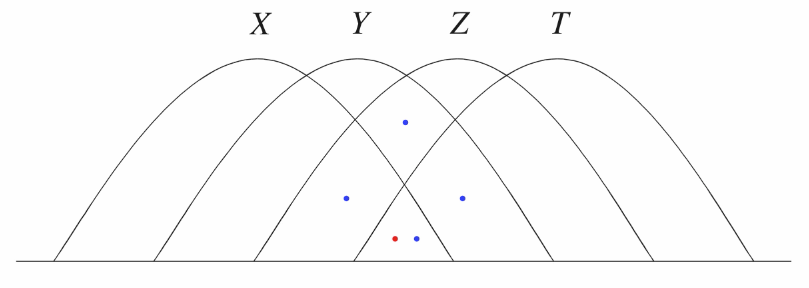
\includegraphics[width=0.5\linewidth]{imgs/exp3_17.png}
    \caption{Shannon's Perfect Secrecy Theorem}
    \label{fig:my_label}
\end{figure}

\newpage
\section{Zero-Error Data Compression}
\begin{itemize}
    \item Why $H(X)$ measures the amount of information in $X$?
    \item A first look at data compression: Prefix codes
    \item How to construct optimal prefix codes - Huffman codes?
\end{itemize}

\subsection{The Entropy Bound}

\paragraph{Definition 4.1} A D-ary source code $\mathcal{C}$ for a source random variable $X$ is a mapping from $\mathcal{X}$ to $\mathcal{D}^{*},$ the set of all finite length sequences of symbols taken from a $D$ -ary code alphabet.

\paragraph{Definition 4.2} $\mathrm{A}$ code $\mathcal{C}$ is uniquely decodable if for any finite source sequence, the sequence of code symbols corresponding to this source sequence is different from the sequence of code symbols corresponding to any other (finite) source sequence.

\paragraph{Example 4.3} Let $\mathcal{X}=\{A, B, C, D\} .$ Consider the code $\mathcal{C}$ defined by
$$
\begin{array}{c|c}
x & \mathcal{C}(x) \\
\hline \mathrm{A} & 0 \\
\mathrm{B} & 1 \\
\mathrm{C} & 01 \\
\mathrm{D} & 10
\end{array}
$$
$$
\begin{array}{ll}
A A D & \rightarrow 0010 \\
A C A & \rightarrow 0010 \\
A A B A & \rightarrow 0010
\end{array}
$$
Therefore, $\mathcal{C}$ not uniquely decodable.

\begin{tcolorbox}
\paragraph{Theorem 4.4 (Kraft Inequality)} Let $\mathcal{C}$ be a $D$ -ary source code, and let $l_{1}, l_{2}, \cdots, l_{m}$ be the lengths of the codewords. If $\mathcal{C}$ is uniquely decodable, then
$$
\sum_{k=1}^{m} D^{-l_{k}} \leq 1
$$
\end{tcolorbox}
\paragraph{Proof}
1. Without loss of generality, assume
$$
l_{1} \leq l_{2} \leq \cdots \leq l_{m}
$$
2. Let $N$ be an arbitrary positive integer, and consider
$$
\left(\sum_{k=1}^{m} D^{-l_{k}}\right)^{N}
= \sum_{k_{1}=1}^{m} \sum_{k_{2}=1}^{m} \ldots \sum_{k_{N}=1}^{m} D^{-\left(l_{k_{1}}+l_{k_{2}}+\cdots+l_{k_{N}}\right)}
$$
3. By collecting terms of the same degree on the $\mathrm{RHS}$, we write
$$
\left(\sum_{k=1}^{m} D^{-l} k\right)^{N}=\sum_{i=1}^{N l m} A_{i} D^{-i}
$$
where $A_{i}$ is the coefficient of $D^{-i}$ on the LHS.

4. Now observe that $A_{i}$ gives the total number of sequences of $N$ codewords with a total length of $i$ code symbols. Since the code is uniquely decodable, these code sequences must be distinct, and therefore
$$
A_{i} \leq D^{i}
$$
because there are $D^{i}$ distinct sequences of $i$ code symbols.
5. Substitute and we have
$$
\left(\sum_{k=1}^{m} D^{-l_{k}}\right)^{N} \leq \sum_{i=1}^{N l m} D^{i} D^{-i}=\sum_{i=1}^{N l_{m}} 1=N l_{m}
$$
or
$$
\sum_{k=1}^{m} D^{-l} k \leq\left(N l_{m}\right)^{1 / N}
$$
since this inequality holds for any $N,$ upon letting $N \rightarrow \infty,$ we obtain $(1),$ completing the proof.


\begin{tcolorbox}
\paragraph{Theorem 4.6 (Entropy Bound)} Let $\mathcal{C}$ be a $D$ -ary uniquely decodable code for a source random variable $X$ with entropy $H_{D}(X) .$ Then the expected length of $\mathcal{C}$ is lower bounded by $H_{D}(X),$ i.e.
$$
L \geq H_{D}(X)
$$
This lower bound is tight if and only if $l_{i}=-\log _{D} p_{i}$ for all $i$
\end{tcolorbox}

\paragraph{Proof}
1. since $\mathcal{C}$ is uniquely decodable, the lengths of its codewords satisfy the Kraft inequality. Write
$$
L=\sum_{i} p_{i} l_{i}=\sum_{i} p_{i} \log _{D} D^{l_{i}}
$$
and recall that
$$
H_{D}(X)=-\sum_{i} p_{i} \log _{D} p_{i}
$$
Then 
$$
\begin{aligned}
L-H_{D}(X) &=\sum_{i} p_{i}\left(\log _{D} p_{i}+\log _{D} D^{l} i\right) \\
&=\sum_{i} p_{i} \log _{D}\left(p_{i} D^{l} i\right) \\
&=(\ln D)^{-1} \sum_{i} p_{i} \ln \left(p_{i} D^{l} i\right) \\
& \geq(\ln D)^{-1} \sum_{i} p_{i}\left(1-\frac{1}{p_{i} D^{l} i}\right) \qquad (\text{fundamental inequality:}  \quad \ln a \geq 1-\frac{1}{a} \quad\left(a=p_{i} D^{l} i\right))\\
&=(\ln D)^{-1} \sum_{i}\left(p_{i}-D^{-l} i\right) \\
&\geq(\ln D)^{-1}\left[1-\sum_{i} D^{-l} i\right] \\
&=0
\end{aligned}
$$
The inequality bounds hold tight if and only if $p_{i} D^{l_{i}}=1, \text { or } l_{i}=-\log _{D} p_{i}$ for all $i$. If this holds, we have
$$
\sum_{i} D^{-l_{i}}=\sum_{i} D^{\log _{D} p_{i}}=\sum_{i} p_{i}=1
$$

\begin{tcolorbox}
\paragraph{Corollary 4.7 (Theorem 2.43)} $H(X) \leq \log |\mathcal{X}|$.
\end{tcolorbox}
\paragraph{Proof} Let $\mathcal{X}=\{0,1, \cdots,|\mathcal{X}|-1\}$. Let $\mathcal{C}$ be the identity code, i.e.,
$$
\begin{array}{c|cccc|c}
x & 0 & 1 & \cdots & |\mathcal{X}|-1 \\
\hline \mathcal{C}(x) & 0 & 1 & \cdots & |\mathcal{X}|-1
\end{array}
$$
Evidently, $\mathcal{C}$ is an $|\mathcal{X}|$ -ary uniquely decodable code, with expected length equals $1 .$
By the entropy bound, we have
$$
1=L \geq H_{|\mathcal{X}|}(X)
$$
Leaving the base unspecified, we have
$$
H(X) \leq \log |\mathcal{X}|
$$

\begin{tcolorbox}
\paragraph{Definition 4.8} The redundancy $R$ of a $D$ -ary uniquely decodable code is the difference between the expected length of the code and the entropy of the source.
By the entropy bound,
$$
R=L-H_{D}(X) \geq 0
$$
\end{tcolorbox}

\newpage
\subsection{Prefix Codes}
\paragraph{Definition 4.9} A code is called a prefix-free code if no codeword is a prefix of any other codeword. For brevity, a prefix-free code will be referred to as a prefix code.

\paragraph{Code Tree for Prefix Code}
\begin{itemize}
    \item A D-ary tree is a graphical representation of a collection of finite sequences of $D$ -ary symbols.
    \item A node is either an internal node or a leaf.
    \item The tree representation of a prefix code is called a code tree.
\end{itemize}

\begin{figure}[!h]
    \centering
    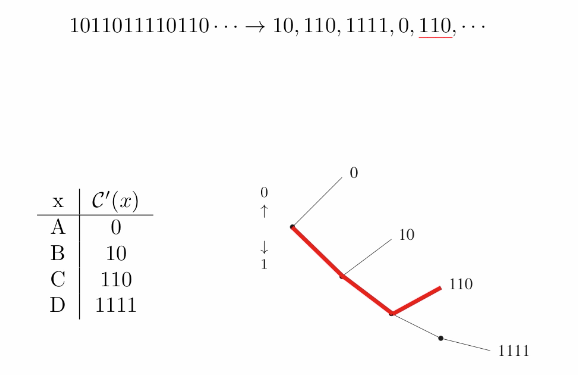
\includegraphics[width=0.5\linewidth]{imgs/exp4_10.png}
    \caption{Instantaneous Decoding}
    \label{fig:my_label}
\end{figure}

\begin{tcolorbox}
\paragraph{Theorem 4.11} There exists a $D$-ary prefix code with codeword lengths $l_{1}$ $l_{2}, \cdots, l_{m}$ if and only if the Kraft inequality
$$
\sum_{k=1}^{m} D^{-l_{k}} \leq 1
$$
is satisfied.
\end{tcolorbox}
\paragraph{Proof}
Direct part follows because a prefix code is uniquely decodable and hence satisfies Kraft's inequality.

(Converse)
1. We need to prove the existence of a D-ary prefix code with codeword lengths $l_{1}, l_{2}, \cdots, l_{m}$ if these lengths satisfy the Kraft inequality. Without loss of generality, assume that
$$
l_{1} \leq l_{2} \leq \cdots \leq l_{m}
$$

2. Consider all the $D$-ary sequences of lengths less than or equal to $l_{m}$ and regard them as the nodes of the full D-ary tree of depth $l_{m}$. We will refer to a sequence of length $l$ as a node of order $l$.

3. There are $D^{l_1}>1$ (since $l_{1} \geq 1$ ) nodes of order $l_{1}$ which can be chosen as the first codeword. Thus choosing the first codeword is always possible.

4. Assume that the first $i$ codewords have been chosen successfully, where $1 \leq i \leq m-1,$ and we want to choose a node of order $l_{i+1}$ as the $(i+1)$ st codeword such that it is not prefixed by any of the previously chosen codewords.

5. Since all the previously chosen codewords are not prefixes of each other, their descendants of order $l_{i+1}$ do not overlap. The $(i+1)$ st node to be chosen cannot be a descendant of any of the previously chosen codewords. Therefore, the number of nodes which can be chosen as the $(i+1)$ st codeword is
$$
D^{l_{i}+1}-D^{l_{i}+1}-l_{1}-D^{l_{i}+1}-l_{2}-\ldots-D^{l_{i}+1}-l_{i}
$$

6. If $l_{1}, l_{2}, \cdots, l_{m}$ satisfy the Kraft inequality, we have
$$
D^{-l_{1}}+\cdots+D^{-l_{i}}+D^{-l_{i+1}} \leq 1
$$
7. Multiplying by $D^{l} i+1,$ we have
$$
D^{l_{i+1}-l_{1}}+\cdots+D^{l_{i}+1}-l_{i}+D^{l_{i+1}-l_{i+1}} \leq D^{l_{i}+1}
$$
Or
$$
D^{l_{i+1}}-D^{l_{i+1} -l_1}-\cdots-D^{l_{i+1} -l_i} \geq 1
$$
Thus we have shown by induction the existence of a prefix code with codeword lengths $l_{1}, l_{2}, \cdots, l_{m}$ completing the proof.

\paragraph{Definition ($D$-adic distribution)}
\begin{itemize}
    \item $p_{i}=D^{-t_{i}}$ for all $i,$ where $t_{i}$ is integer
    \item dyadic when $D=2$
\end{itemize}
\begin{tcolorbox}
\paragraph{Corollary 4.12} There exists a $D$-ary prefix code which achieves the entropy bound for a distribution $\left\{p_{i}\right\}$ if and only if $\left\{p_{i}\right\}$ is $D$-adic.
\end{tcolorbox}

\subsection{Huffman Codes}
A simple construction of optimal prefix codes.
\begin{itemize}
    \item Binary Case: Keep merging the two smallest probability masses until one probability mass (i.e., 1 ) is left.
    \item D-ary Case: Insert zero probability masses until there are $D+k(D-1)$ masses (if necessary). Keep merging the $D$ smallest probability masses until one probability mass (i.e., 1 ) is left.
    \item In general there can be more than one Huffman code.
\end{itemize}
\begin{figure}[!h]
    \centering
    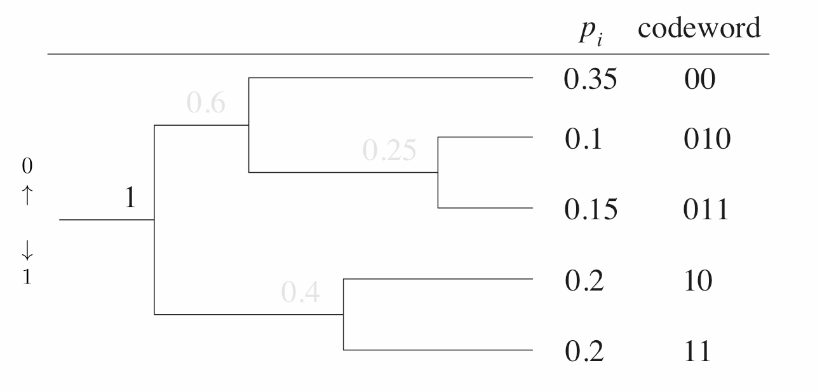
\includegraphics[width=0.5\linewidth]{imgs/exp4_16.png}
    \caption{Instantaneous Decoding}
    \label{fig:my_label}
\end{figure}

\paragraph{Optimality of Huffman Codes}
\begin{itemize}
    \item Without loss of generality, assume $p_{1} \geq p_{2} \geq \cdots \geq p_{m}$
    \item Denote the codeword assigned to $p_{i}$ by $c_{i},$ and its length by $l_{i}$
\end{itemize}

\begin{tcolorbox}
\paragraph{Theorem 4.17} The Huffman procedure produces an optimal prefix code.
\\
\paragraph{Lemma 4.15} In an optimal code, shorter codewords are assigned to larger probabilities, i.e.,
$$
l_{1} \leq l_{2} \leq \cdots \leq l_{m}
$$
\paragraph{Lemma 4.16} There exists an optimal code in which the codewords assigned to the two smallest probabilities are siblings, i.e., the two codewords have the same length and they differ only in the last symbol.

\end{tcolorbox}
\paragraph{Proof}
1. Consider a probability distribution
$$
\left\{p_{1}, \cdots, p_{i}, \cdots, p_{j}, \cdots p_{m}\right\}
$$
such that $p_{i}>p_{j}$. Assume that in a particular code, the codewords $c_{i}$ and $c_{j}$ are such that $l_{i}>l_{j},$ i.e., a shorter codeword is assigned to a smaller probability.
2. Intuitively, by exchanging $c_{i}$ and $c_{j},$ the expected length of the code should be improved.
3. Specifically, let
$$
L=\sum_{k} p_{k} l_{k}=\sum_{k \neq i, j} p_{k} l_{k}+\left(p_{i} l_{i}+p_{j} l_{j}\right)
$$
be the expected length of the code, and
$$
L^{\prime}=\sum_{k \neq i, j} p_{k} l_{k}+\left(p_{i} l_{j}+p_{j} l_{i}\right)
$$
be the expected length of the code obtained by exchanging $c_{i}$ and $c_{j}$

4. Comparing $L^{\prime}$ and $L$, we see that
$$
\begin{aligned}
L^{\prime}-L &=\left(p_{i} l_{j}+p_{j} l_{i}\right)-\left(p_{i} l_{i}+p_{j} l_{j}\right) \\
&=\left(p_{i} l_{j}-p_{i} l_{i}\right)-\left(p_{j} l_{j}-p_{j} l_{i}\right) \\
&=p_{i}\left(l_{j}-l_{i}\right)-p_{j}\left(l_{j}-l_{i}\right) \\
&=\left(p_{i}-p_{j}\right)\left(l_{j}-l_{i}\right)
\end{aligned}
$$
This is negative because $p_{i}>p_{j}$ and $l_{i}>l_{j} .$ Therefore, $L^{\prime}<L$
5. Since the original code can be improved, it is not an optimal code.
6. Therefore, for an optimal code, shorter codewords are assigned to larger probabilities. The lemma is proved.

\newpage
\section{Strong Typicality}
\subsection{Strong AEP}
\begin{tcolorbox}
\paragraph{Definition 6.1}  The strongly typical set $T_{[X] \delta}^{n}$ with respect to $p(x)$ is the set
of sequences $x = (x_1,x_2, \cdots  ,x_n) \in X_n$ such that $N(x ; \mathbf{x})=0$ for $x \notin \mathcal{S}_{X}$ and
\begin{equation}
	\sum_{x}\left|\frac{1}{n} N(x ; \mathbf{x})-p(x)\right| \leq \delta
\end{equation}
where $N(x ; \mathbf{x})$ is the number of occurrences of $x$ in the sequence $ \mathbf{x}$ and $\delta$ is an arbitrarily small positive real number. The sequences in $T_{[X] \delta}^{n}$ are called
strongly $\delta$-typical sequences.
\end{tcolorbox}

\begin{tcolorbox}
\paragraph{Theorem 6.2 (Strong AEP)} There exists $\eta>0$ such that $\eta \rightarrow 0$ as $\delta \rightarrow 0$, and the following hold:\\
1) If $\mathbf{x} \in T_{[X] \delta}^{n}$, then
$$
2^{-n(H(X)+\eta)} \leq p(\mathbf{x}) \leq 2^{-n(H(X)-\eta)}
$$
2) For $n$ sufficiently large,
$$
\operatorname{Pr}\left\{\mathbf{X} \in T_{[X] \delta}^{n}\right\}>1-\delta
$$
3) For $n$ sufficiently large,
$$
(1-\delta) 2^{n(H(X)-\eta)} \leq\left|T_{[X] \delta}^{n}\right| \leq 2^{n(H(X)+\eta)}
$$
\end{tcolorbox}

\paragraph{Proof.} 
\begin{enumerate}
	\item To prove Property $1,$ for $\mathbf{x} \in T_{[X] \delta}^{n},$ we write
$$
\begin{aligned}
	p(\mathbf{x})&=\prod_{x} p(x)^{N(x ; \mathbf{x})} \\
	\log p(\mathbf{x})
	&=\sum_{x} N(x ; \mathbf{x}) \log p(x) \\
	&=\sum_{x}(N(x ; \mathbf{x})-n p(x)+n p(x)) \log p(x) \\
	&=n \sum_{x} p(x) \log p(x)-n \sum_{x}\left(\frac{1}{n} N(x ; \mathbf{x})-p(x)\right)(-\log p(x)) \\
	&=-n\left[H(X)+\sum_{x}\left(\frac{1}{n} N(x ; \mathbf{x})-p(x)\right)(-\log p(x))\right]
\end{aligned}
$$
Since $\mathbf{x} \in T_{[X] \delta}^{n}$
$$
\sum_{x}\left|\frac{1}{n} N(x ; \mathbf{x})-p(x)\right| \leq \delta
$$
which implies

$$
\begin{aligned}
	\left|\sum_{x}\left(\frac{1}{n} N(x ; \mathbf{x})-p(x)\right)(-\log p(x))\right|
	& \leq \sum_{x}\left|\frac{1}{n} N(x ; \mathbf{x})-p(x)\right|(-\log p(x)) \\
	&\leq-\log \left(\min _{x} p(x)\right) \sum_{x}\left|\frac{1}{n} N(x ; \mathbf{x})-p(x)\right| \\
	&\leq-\delta \log \left(\min _{x} p(x)\right) \\
	&=\eta > 0
\end{aligned}
$$
Therefore,
$$
-\eta \leq \sum_{x}\left(\frac{1}{n} N(x ; \mathbf{x})-p(x)\right)(-\log p(x)) \leq \eta
$$
It then follows from (6.9) that
$$-n(H(X)+\eta) \leq \log p(\mathbf{x}) \leq-n(H(X)-\eta)$$
$$2^{-n(H(X)+\eta)} \leq p(\mathbf{x}) \leq 2^{-n(H(X)-\eta)}$$
where $\eta \rightarrow 0$ as $\delta \rightarrow 0$, proving Property 1.\\

\item To prove Property 2, we write
$N(x ; \mathbf{X})=\sum_{k=1}^{n} B_{k}(x)$ 
$$B_{k}(x)=\left\{\begin{array}{l}1 \text { if } X_{k}=x \\ 0 \text { if } X_{k} \neq x\end{array}\right.$$
Then $B_{k}(x), k=1,2, \cdots, n$ are i.i.d. random variables with
$$
\operatorname{Pr}\left\{B_{k}(x)=1\right\}=p(x)
$$
and
$$
\operatorname{Pr}\left\{B_{k}(x)=0\right\}=1-p(x)
$$
Note that
$$
E B_{k}(x)=(1-p(x)) \cdot 0+p(x) \cdot 1=p(x)
$$
By the weak law of large numbers, for any $\delta>0$ and for any $x \in \mathcal{X}$
$$
\operatorname{Pr}\left\{\left|\frac{1}{n} \sum_{k=1}^{n} B_{k}(x)-p(x)\right|>\frac{\delta}{|\mathcal{X}|}\right\}<\frac{\delta}{|\mathcal{X}|}
$$
for $n$ sufficiently large. Then
$$
\begin{aligned}
	\operatorname{Pr}\left\{\left|\frac{1}{n} N(x ; \mathbf{X})-p(x)\right|>\frac{\delta}{|\mathcal{X}|} \text { for some } x\right\} 
	&=\operatorname{Pr}\left\{\left|\frac{1}{n} \sum_{k=1}^{n} B_{k}(x)-p(x)\right|>\frac{\delta}{|\mathcal{X}|} \text { for some } x\right\} \\
	&=\operatorname{Pr}\left\{\bigcup_{x}\left\{\left|\frac{1}{n} \sum_{k=1}^{n} B_{k}(x)-p(x)\right|>\frac{\delta}{|\mathcal{X}|}\right\}\right\} \\
	&\leq \sum_{x} \operatorname{Pr}\left\{\left|\frac{1}{n} \sum_{k=1}^{n} B_{k}(x)-p(x)\right|>\frac{\delta}{|\mathcal{X}|}\right\} \\
	&<\sum_{x} \frac{\delta}{|\mathcal{X}|} =\delta
\end{aligned}
$$
where we have used the union bound ($\operatorname{Pr}\{A \cup B\} \leq \operatorname{Pr}\{A\}+\operatorname{Pr}\{B\}$) to obtain $(6.27) .$ since
$$
\sum_{x}\left|\frac{1}{n} N(x ; \mathbf{x})-p(x)\right|>\delta
$$
implies
$$
\left|\frac{1}{n} N(x ; \mathbf{x})-p(x)\right|>\frac{\delta}{|\mathcal{X}|} \quad \text { for some } x \in \mathcal{X}
$$
we have
$$
\begin{aligned}
	\operatorname{Pr}\left\{\mathbf{X} \in T_{[X] \delta}^{n}\right\} 
	&=\operatorname{Pr}\left\{\sum_{x}\left|\frac{1}{n} N(x ; \mathbf{X})-p(x)\right| \leq \delta\right\} \\
	&=1-\operatorname{Pr}\left\{\sum_{x}\left|\frac{1}{n} N(x ; \mathbf{X})-p(x)\right|>\delta\right\} \\
	&\geq 1-\operatorname{Pr}\left\{\left|\frac{1}{n} N(x ; \mathbf{X})-p(x)\right|>\frac{\delta}{|\mathcal{X}|} \text { for some } x \in \mathcal{X}\right\} \\
	&>1-\delta
\end{aligned}
$$
proving Property 2 .

\paragraph{\textcolor{red}{Homework}}
2. Let $\mathbf{X}=\left(X_{1}, X_{2}, \cdots, X_{n}\right),$ where $X_{k}$ are i.i.d. with generic random variable $X .$ Prove that
$$
\operatorname{Pr}\left\{\mathbf{X} \in T_{[X] \delta}^{n}\right\} \geq 1-\frac{|\mathcal{X}|^{3}}{n \delta^{2}}
$$
for any $n$ and $\delta>0 .$ This shows that $\operatorname{Pr}\left\{\mathbf{X} \in T_{[X] \delta}^{n}\right\} \rightarrow 1$ as $\delta \rightarrow 0$ and $n \rightarrow \infty$ if $\sqrt{n} \delta \rightarrow \infty$
\paragraph{\textcolor{red}{Proof.}}
$$
\begin{aligned}
	\operatorname{Pr}\left\{\mathbf{X} \in T_{[X] \delta}^{n}\right\} 
	&=\operatorname{Pr}\left\{\sum_{x}\left|\frac{1}{n} N(x ; \mathbf{X})-p(x)\right| \leq \delta\right\} \\
	&=1-\operatorname{Pr}\left\{\sum_{x}\left|\frac{1}{n} N(x ; \mathbf{X})-p(x)\right|>\delta\right\} \\
	&\geq 1-\operatorname{Pr}\left\{\left|\frac{1}{n} N(x ; \mathbf{X})-p(x)\right|>\frac{\delta}{|\mathcal{X}|} \text { for some } x \in \mathcal{X}\right\} \\
%	&>1-\delta
\end{aligned}
$$

$$
\begin{aligned}
	\operatorname{Pr}\left\{\left|\frac{1}{n} N(x ; \mathbf{X})-p(x)\right|>\frac{\delta}{|\mathcal{X}|} \text { for some } x\right\} 
	&=\operatorname{Pr}\left\{\left|\frac{1}{n} \sum_{k=1}^{n} B_{k}(x)-p(x)\right|>\frac{\delta}{|\mathcal{X}|} \text { for some } x\right\} \\
	&=\operatorname{Pr}\left\{\bigcup_{x}\left\{\left|\frac{1}{n} \sum_{k=1}^{n} B_{k}(x)-p(x)\right|>\frac{\delta}{|\mathcal{X}|}\right\}\right\} \\
	&\leq \sum_{x} \operatorname{Pr}\left\{\left|\frac{1}{n} \sum_{k=1}^{n} B_{k}(x)-p(x)\right|>\frac{\delta}{|\mathcal{X}|}\right\}  \qquad \text{(i.i.d)}\\
	&\leq \sum_{x} \operatorname{Pr}\left\{\left| B_{k}(x)-p(x)\right|>\frac{\delta}{|\mathcal{X}|}\right\} \\
	&<\sum_{x} \frac{\sigma^{2}   |\mathcal{X}|^2 }{n \delta^{2}} \\
	&< \frac{|\mathcal{X}|^{3}}{n \delta^{2}}
%	&<\sum_{x} \frac{\delta}{|\mathcal{X}|} =\delta
\end{aligned}
$$
Using Chebyshev's inequality
$$
\mathrm{P}\left(\left|\bar{X}_{n}-\mu\right| \geq \varepsilon\right) \leq \frac{\sigma^{2}}{n \varepsilon^{2}}
$$
Therefore we proved
$$
\operatorname{Pr}\left\{\mathbf{X} \in T_{[X] \delta}^{n}\right\} \geq 1-\frac{|\mathcal{X}|^{3}}{n \delta^{2}}
$$
\begin{tcolorbox}
\paragraph{Theorem 6.3.} For sufficiently large $n,$ there exists $\varphi(\delta)>0$ such that
$$
\operatorname{Pr}\left\{\mathbf{X} \notin T_{[X] \delta}^{n}\right\}<2^{-n \varphi(\delta)}
$$
\end{tcolorbox}
The proof of this theorem is based on the Chernoff bound [66] which we prove in the next lemma.

Apply Lemma 6.4.
$$
\begin{aligned}
	\log \operatorname{Pr}\left\{\sum_{k=1}^{n} B_{k}(x) \geq n(p(x)+\delta)\right\}
	&\leq-\operatorname{sn}(p(x)+\delta)+\log E\left[2^{s \sum_{k=1}^{n} B_{k}(x)}\right] \\
	&\stackrel{a)}{=}-\operatorname{sn}(p(x)+\delta)+\log \left(\prod_{k=1}^{n} E\left[2^{s B_{k}(x)}\right]\right) \\
	&\stackrel{b)}{=}-\operatorname{sn}(p(x)+\delta)+n \log \left(1-p(x)+p(x) 2^{s}\right) \\
	&\stackrel{c)}{\leq}-\operatorname{sn}(p(x)+\delta)+n(\ln 2)^{-1}\left(-p(x)+p(x) 2^{s}\right) \\
	&=-n\left[s(p(x)+\delta)+(\ln 2)^{-1} p(x)\left(1-2^{s}\right)\right]
\end{aligned}
$$
where\\
(a) follows because $B_{k}(x)$ are mutually independent;\\
(b) is a direct evaluation of the expectation from the definition of $B_{k}(x)$ in (6.20)\\
(c) follows from the fundamental inequality $\ln a \leq a-1$\\
In $(6.48),$ upon defining
$$
\beta_{x}(s, \delta)=s(p(x)+\delta)+(\ln 2)^{-1} p(x)\left(1-2^{s}\right)
$$
we have
$$
\log \operatorname{Pr}\left\{\sum_{k=1}^{n} B_{k}(x) \geq n(p(x)+\delta)\right\} \leq-n \beta_{x}(s, \delta)
$$
Or
$$
\operatorname{Pr}\left\{\sum_{k=1}^{n} B_{k}(x) \geq n(p(x)+\delta)\right\} \leq 2^{-n \beta_{x}(s, \delta)}
$$

$$
\begin{aligned}
	\operatorname{Pr}\left\{\left|\frac{1}{n} \sum_{k=1}^{n} B_{k}(x)-p(x)\right| \geq \delta\right\}
	&=\operatorname{Pr}\left\{\left|\sum_{k=1}^{n} B_{k}(x)-n p(x)\right| \geq n \delta\right\} \\
	&\leq \operatorname{Pr}\left\{\sum_{k=1}^{n} B_{k}(x) \geq n(p(x)+\delta)\right\} +\operatorname{Pr}\left\{\sum_{k=1}^{n} B_{k}(x) \leq n(p(x)-\delta)\right\} \\
	&\leq 2^{-n \beta_{x}(s, \delta)}+2^{-n \sigma_{x}(s, \delta)} \\
	&\leq 2 \cdot 2^{-n \min \left(\beta_{x}(s, \delta), \sigma_{x}(s, \delta)\right)} \\
	&=2^{-n\left[\min \left(\beta_{x}(s, \delta), \sigma_{x}(s, \delta)\right)-\frac{1}{n}\right]} \\
	&=2^{-n \varphi_{x}(\delta)}
\end{aligned}
$$
where
$$
\varphi_{x}(\delta)=\min \left(\beta_{x}(s, \delta), \sigma_{x}(s, \delta)\right)-\frac{1}{n}
$$

$$
\begin{aligned}
	\operatorname{Pr}\left\{\mathbf{X} \in T_{[X] \delta}^{n}\right\} 
	&=\operatorname{Pr}\left\{\sum_{x}\left|\frac{1}{n} N(x ; \mathbf{X})-p(x)\right| \leq \delta\right\} \\
	&\geq \operatorname{Pr}\left\{\left|\frac{1}{n} N(x ; \mathbf{X})-p(x)\right| \leq \frac{\delta}{|\mathcal{X}|} \text { for all } x \in \mathcal{X}\right\} \\
	&=1-\operatorname{Pr}\left\{\left|\frac{1}{n} N(x ; \mathbf{X})-p(x)\right|>\frac{\delta}{|\mathcal{X}|} \text { for some } x \in \mathcal{X}\right\} \\
	&\geq 1-\sum_{x} \operatorname{Pr}\left\{\left|\frac{1}{n} N(x ; \mathbf{X})-p(x)\right|>\frac{\delta}{|\mathcal{X}|}\right\} \\
	&= 1-\sum_{x} \operatorname{Pr}\left\{\left|\frac{1}{n} \sum_{k=1}^{n} B_{k}(x)-p(x)\right|>\frac{\delta}{|\mathcal{X}|}\right\} \\
	&= 1-\sum_{x: p(x)>0} \operatorname{Pr}\left\{\left|\frac{1}{n} \sum_{k=1}^{n} B_{k}(x)-p(x)\right|>\frac{\delta}{|\mathcal{X}|}\right\} \\
	&\geq 1-\sum_{x: p(x)>0} 2^{-n \varphi_{x}\left(\frac{\delta}{|x|}\right)}
\end{aligned}
$$

\begin{tcolorbox}
\paragraph{Lemma 6.4 (Chernoff Bound).} Let $Y$ be a real random variable and $s$ be any nonnegative real number. Then for any real number a,
$$
\log \operatorname{Pr}\{Y \geq a\} \leq-s a+\log E\left[2^{s Y}\right]
$$
and
$$
\log \operatorname{Pr}\{Y \leq a\} \leq s a+\log E\left[2^{-s Y}\right]
$$
\end{tcolorbox}
\paragraph{Proof}. Let
$$
u(y)=\left\{\begin{array}{l}
	1 \text { if } y \geq 0 \\
	0 \text { if } y<0
\end{array}\right.
$$
Then for any $s \geq 0$
$$
u(y-a) \leq 2^{s(y-a)}
$$
Taking expectation on both sides
$$
E[u(Y-a)] \leq E\left[2^{s(Y-a)}\right]=2^{-s a} E\left[2^{s Y}\right]
$$
since
$$
E[u(Y-a)]=\operatorname{Pr}\{Y \geq a\} \cdot 1+\operatorname{Pr}\{Y<a\} \cdot 0=\operatorname{Pr}\{Y \geq a\}
$$
we see that
$$
\operatorname{Pr}\{Y \geq a\} \leq 2^{-s a} E\left[2^{s Y}\right]=2^{-s a+\log E\left[2^{s Y}\right]}
$$

\end{enumerate}

\subsection{Strong Typicality Versus Weak Typicality}
We will prove in the next proposition that strong typicality is
stronger than weak typicality in the sense that the former implies the latter
\begin{tcolorbox}
\paragraph{Proposition 6.5.} For any $\mathbf{x} \in \mathcal{X}^{n},$ if $\mathbf{x} \in T_{[X] \delta}^{n},$ then $\mathbf{x} \in W_{[X] \eta}^{n},$ where $\eta \rightarrow 0$ as $\delta \rightarrow 0$
\end{tcolorbox}

\paragraph{Proof.} By Property 1 of strong AEP (Theorem 6.2$),$ if $\mathbf{x} \in T_{[X] \delta}^{n},$ then
$$
2^{-n(H(X)+\eta)} \leq p(\mathbf{x}) \leq 2^{-n(H(X)-\eta)}
$$
Or
$$
H(X)-\eta \leq-\frac{1}{n} \log p(\mathbf{x}) \leq H(X)+\eta
$$
where $\eta \rightarrow 0$ as $\delta \rightarrow 0 .$ Then $\mathbf{x} \in W_{[X] \eta}^{n}$ by Definition $5.2 .$ The proposition is proved.

\subsection{Joint Typicality}
Consider a bivariate information source $\left\{\left(X_{k}, Y_{k}\right), k \geq 1\right\}$ where $\left(X_{k}, Y_{k}\right)$ are i.i.d. with distribution $p(x, y) .$ We use $(X, Y)$ to denote the pair of generic random variables.
\begin{tcolorbox}
\paragraph{Definition $6.6 .$} The strongly jointly typical set $T_{[X Y] \delta}^{n}$ with respect to $p(x, y)$ is the set of $(\mathbf{x}, \mathbf{y}) \in \mathcal{X}^{n} \times \mathcal{Y}^{n}$ such that $N(x, y ; \mathbf{x}, \mathbf{y})=0$ for $(x, y) \notin \mathcal{S}_{X Y}$
and
$$
\sum_{x} \sum_{y}\left|\frac{1}{n} N(x, y ; \mathbf{x}, \mathbf{y})-p(x, y)\right| \leq \delta
$$
where $N(x, y ; \mathbf{x}, \mathbf{y})$ is the number of occurrences of $(x, y)$ in the pair of sequences $(\mathbf{x}, \mathbf{y})$ and $\delta$ is an arbitrarily small positive real number. $A$ pair of sequences $(\mathbf{x}, \mathbf{y})$ is called strongly jointly $\delta$ -typical if it is in $T_{[X Y] \delta}^{n}$
\end{tcolorbox}

\begin{tcolorbox}
\paragraph{Theorem 6.7 (Consistency).} If $(\mathbf{x}, \mathbf{y}) \in T_{[X Y] \delta}^{n},$ then $\mathbf{x} \in T_{[X] \delta}^{n}$ and $\mathbf{y} \in T_{[Y] \delta}^{n}$
\end{tcolorbox}
\paragraph{Proof.} If $(\mathbf{x}, \mathbf{y}) \in T_{[X Y] \delta}^{n},$ then
$$
\sum_{x} \sum_{y}\left|\frac{1}{n} N(x, y ; \mathbf{x}, \mathbf{y})-p(x, y)\right| \leq \delta
$$
Upon observing that
$$
N(x ; \mathbf{x})=\sum_{y} N(x, y ; \mathbf{x}, \mathbf{y})
$$
we have
$$
\begin{aligned}
	\sum_{x}\left|\frac{1}{n} N(x ; \mathbf{x})-p(x)\right| 
	&=\sum_{x}\left|\frac{1}{n} \sum_{y} N(x, y ; \mathbf{x}, \mathbf{y})-\sum_{y} p(x, y)\right| \\
	&=\sum_{x}\left|\sum_{y}\left(\frac{1}{n} N(x, y ; \mathbf{x}, \mathbf{y})-p(x, y)\right)\right| \\
	&\leq \sum_{x} \sum_{y}\left|\frac{1}{n} N(x, y ; \mathbf{x}, \mathbf{y})-p(x, y)\right| \\
	&\leq \delta
\end{aligned}
$$
Therefore, $\mathbf{x} \in T_{[X] \delta^{*}}^{n}$ Similarly, $\mathbf{y} \in T_{[Y] \delta}^{n} .$ The theorem is proved.
\begin{tcolorbox}
\paragraph{Theorem 6.8 (Preservation).} 
Let $Y=f(X) $. If
$$
\mathbf{x}=\left(x_{1}, x_{2}, \cdots, x_{n}\right) \in T_{[X] \delta}^{n}
$$
then
$$
f(\mathbf{x})=\left(y_{1}, y_{2}, \cdots, y_{n}\right) \in T_{[Y] \delta}^{n}
$$
where $y_{i}=f\left(x_{i}\right)$ for $1 \leq i \leq n$
\end{tcolorbox}
\paragraph{Proof.} Consider $\mathbf{x} \in T_{[X] \delta}^{n},$ i.e.,
$$
\sum_{x}\left|\frac{1}{n} N(x ; \mathbf{x})-p(x)\right|<\delta
$$
since $Y=f(X)$
$$
p(y)=\sum_{x \in f^{-1}(y)} p(x)
$$
for all $y \in \mathcal{Y}$. On the other hand,
$$
N(y ; f(\mathbf{x}))=\sum_{x \in f^{-1}(y)} N(x ; \mathbf{x})
$$
for all $y \in \mathcal{Y}$. Then
$$
\begin{aligned}
	\sum_{y}\left|\frac{1}{n} N(y ; f(\mathbf{x}))-p(y)\right|
	&=\sum_{y}\left|\sum_{x \in f^{-1}(y)}\left(\frac{1}{n} N(x ; \mathbf{x})-p(x)\right)\right| \\
	&\leq \sum_{y} \sum_{x \in f^{-1}(y)}\left|\frac{1}{n} N(x ; \mathbf{x})-p(x)\right| \\
	&=\sum_{x}\left|\frac{1}{n} N(x ; \mathbf{x})-p(x)\right| \\
	&<\delta
\end{aligned}
$$
Therefore, $f(\mathbf{x}) \in T_{[Y] \delta}^{n},$ proving the lemma.

For a bivariate i.i.d. source $\left\{\left(X_{k}, Y_{k}\right)\right\},$ we have the strong joint asymptotic equipartition property (strong JAEP), which can readily be obtained by applying the strong AEP to the source $\left\{\left(X_{k}, Y_{k}\right)\right\}$.
\begin{tcolorbox}
\paragraph{Theorem 6.9 (Strong JAEP).} Let
$$
(\mathbf{X}, \mathbf{Y})=\left(\left(X_{1}, Y_{1}\right),\left(X_{2}, Y_{2}\right), \cdots,\left(X_{n}, Y_{n}\right)\right)
$$
where$\left(X_{i}, Y_{i}\right)$ are i.i.d. with generic pair of random variables $(X, Y) .$ Then there exists $\lambda>0$ such that $\lambda \rightarrow 0$ as $\delta \rightarrow 0,$ and the following hold:\\
1) If $(\mathbf{x}, \mathbf{y}) \in T_{[X Y] \delta}^{n},$ then
$$
2^{-n(H(X, Y)+\lambda)} \leq p(\mathbf{x}, \mathbf{y}) \leq 2^{-n(H(X, Y)-\lambda)}
$$
2) For $n$ sufficiently large,
$$
\operatorname{Pr}\left\{(\mathbf{X}, \mathbf{Y}) \in T_{[X Y] \delta}^{n}\right\}>1-\delta
$$
3) For $n$ sufficiently large,
$$
(1-\delta) 2^{n(H(X, Y)-\lambda)} \leq\left|T_{[X Y] \delta}^{n}\right| \leq 2^{n(H(X, Y)+\lambda)}
$$
\end{tcolorbox}
From the strong JAEP, we can see the following. since there are approximately $2^{n H(X, Y)}$ typical $(\mathbf{x}, \mathbf{y})$ pairs and approximately $2^{n H(X)}$ typical $\mathbf{x},$ for a typical $\mathbf{x},$ the number of $\mathbf{y}$ such that $(\mathbf{x}, \mathbf{y})$ is jointly typical is approximately
$$
\frac{2^{n H(X, Y)}}{2^{n H(X)}}=2^{n H(Y \mid X)}
$$
on the average. The next theorem reveals that this is not only true on the average, but it is in fact true for every typical $\mathbf{x}$ as long as there exists at least one $\mathbf{y}$ such that $(\mathbf{x}, \mathbf{y})$ is jointly typical.
\begin{tcolorbox}
\paragraph{Theorem 6.10 (Conditional Strong AEP).} For any $\mathrm{x} \in T_{[X] \delta}^{n},$ define
$$
T_{[Y \mid X] \delta}^{n}(\mathbf{x})=\left\{\mathbf{y} \in T_{[Y] \delta}^{n}:(\mathbf{x}, \mathbf{y}) \in T_{[X Y] \delta}^{n}\right\}
$$
If $\left|T_{[Y \mid X] \delta}^{n}(\mathbf{x})\right| \geq 1,$ then
$$
2^{n(H(Y \mid X)-\nu)} \leq\left|T_{[Y \mid X] \delta}^{n}(\mathbf{x})\right| \leq 2^{n(H(Y \mid X)+\nu)}
$$
where $\nu \rightarrow 0$ as $n \rightarrow \infty$ and $\delta \rightarrow 0$
\end{tcolorbox}
\paragraph{Proof.}
Assume that $\left|T_{[Y \mid X] \delta}^{n}(\mathbf{x})\right| \geq 1 .$ We now prove the lower bound on $\left|T_{[Y \mid X] \delta}^{n}(\mathbf{x})\right|$. Let
$$
\{K(x, y),(x, y) \in \mathcal{X} \times \mathcal{Y}\}
$$
be any set of nonnegative integers such thats
$$
\sum_{y} K(x, y)=N(x ; \mathbf{x})
$$
for all $x \in \mathcal{X},$ and for any $\mathbf{y} \in \mathcal{Y}^{n},$ if
$$
N(x, y ; \mathbf{x}, \mathbf{y})=K(x, y)
$$
for all $(x, y) \in \mathcal{X} \times \mathcal{Y},$ then $(\mathbf{x}, \mathbf{y}) \in T_{[X Y] \delta}^{n}$
Then by Definition $6.6,\{K(x, y)\}$ satisfies
$$
\sum_{x} \sum_{y}\left|\frac{1}{n} K(x, y)-p(x, y)\right| \leq \delta
$$
which implies that for all $(x, y) \in \mathcal{X} \times \mathcal{Y},$
$$
\left|\frac{1}{n} K(x, y)-p(x, y)\right| \leq \delta
$$
Or
$$
p(x, y)-\delta \leq \frac{1}{n} K(x, y) \leq p(x, y)+\delta
$$
Straightforward combinatorics reveals that the number of $\mathbf{y}$ which satisfy the constraints in (6.128) is equal to
$$
M(K)=\prod_{x} \frac{N(x ; \mathbf{x}) !}{\prod_{y} K(x, y) !}
$$
and it is readily seen that
$$
\left|T_{[Y \mid X] \delta}^{n}(\mathbf{x})\right| \geq M(K)
$$


\begin{tcolorbox}
\paragraph{Lemma 6.11.} For any $n>0$,
$$
n \ln n-n<\ln n !<(n+1) \ln (n+1)-n
$$
\end{tcolorbox}
Proof. First, we write
$$
\ln n !=\ln 1+\ln 2+\cdots+\ln n
$$
since $\ln x$ is a monotonically increasing function of $x,$ we have
$$
\int_{k-1}^{k} \ln x d x<\ln k<\int_{k}^{k+1} \ln x d x
$$
Summing over $1 \leq k \leq n,$ we have
$$
\int_{0}^{n} \ln x d x<\ln n !<\int_{1}^{n+1} \ln x d x
$$
Or
$$
n \ln n-n<\ln n !<(n+1) \ln (n+1)-n
$$
The lemma is proved.\\

The above theorem says that for any typical $\mathbf{x},$ as long as there is one typical $\mathbf{y}$ such that $(\mathbf{x}, \mathbf{y})$ is jointly typical, there are approximately $2^{n H(Y \mid X)}$ $\mathbf{y}$ such that $(\mathbf{x}, \mathbf{y})$ is jointly typical. This theorem has the following corollary that the number of such typical x grows with $n$ at almost the same rate as the total number of typical $\mathbf{x}$.

\begin{tcolorbox}
\paragraph{Corollary 6.12.} For a joint distribution $p(x, y)$ on $\mathcal{X} \times \mathcal{Y},$ let $S_{[X] \delta}^{n}$ be the set of all sequences $\mathbf{x} \in T_{[X] \delta}^{n}$ such that $T_{[Y \mid X] \delta}^{n}(\mathbf{x})$ is nonempty. Then
$$
\left|S_{[X] \delta}^{n}\right| \geq(1-\delta) 2^{n(H(X)-\psi)}
$$
where $\psi \rightarrow 0$ as $n \rightarrow \infty$ and $\delta \rightarrow 0 .$
\end{tcolorbox}
\paragraph{Proof.} By the consistency of strong typicality (Theorem 6.7$),$ if $(\mathbf{x}, \mathbf{y}) \in$ $T_{[X Y] \delta}^{n},$ then $\mathbf{x} \in T_{[X] \delta}^{n} .$ In particular, $\mathbf{x} \in S_{[X] \delta}^{n} .$ Then
$$
T_{[X Y] \delta}^{n}=\bigcup_{\mathbf{x} \in S_{[X] \delta}^{n}}\left\{(\mathbf{x}, \mathbf{y}): \mathbf{y} \in T_{[Y \mid X] \delta}^{n}(\mathbf{x})\right\}
$$
Using the lower bound on $\left|T_{[X Y] \delta}^{n}\right|$ in Theorem 6.9 and the upper bound on $\left|T_{[Y \mid X] \delta}^{n}(\mathbf{x})\right|$ in the last theorem, we have
$$
(1-\delta) 2^{n(H(X, Y)-\lambda)} \leq\left|T_{[X Y] \delta}^{n}\right| \leq\left|S_{[X] \delta}^{n}\right| 2^{n(H(Y \mid X)+\nu)}
$$
which implies
$$
\left|S_{[X] \delta}^{n}\right| \geq(1-\delta) 2^{n(H(X)-(\lambda+\nu))}
$$
The theorem is proved upon letting $\psi=\lambda+\nu$.

\begin{figure}[!h]
	\centering
	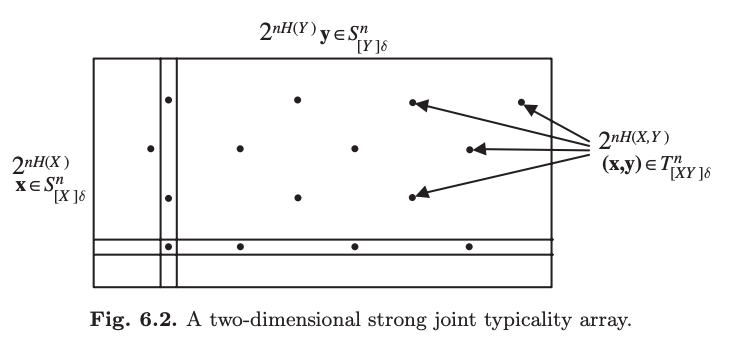
\includegraphics[width=0.7\linewidth]{imgs/exp6_2.png}
	\caption{In this array, the rows and the columns are the typical sequences $\mathbf{x} \in S_{[X] \delta}^{n}$ and $\mathbf{y} \in S_{[Y] \delta}^{n}$ respectively. The total number of rows and columns are approximately equal to $2^{n H(X)}$ and $2^{n H(Y)},$ respectively. An entry indexed by $(\mathbf{x}, \mathbf{y})$ receives a dot if $(\mathbf{x}, \mathbf{y})$ is strongly jointly typical. The total number of dots is approximately equal to $2^{n H(X, Y)}$. The number of dots in each row is approximately equal to $2^{n H(Y \mid X)},$ while the number of dots in each column is approximately equal to $2^{n H(X \mid Y)}$}
	\label{fig:my_label}
\end{figure}

\begin{tcolorbox}
\paragraph{Proposition 6.13.} With respect to a joint distribution $p(x, y)$ on $\mathcal{X} \times \mathcal{Y},$ for any $\delta>0$
$$
\operatorname{Pr}\left\{\mathbf{X} \in S_{[X] \delta}^{n}\right\}>1-\delta
$$
for $n$ sufficiently large.
\end{tcolorbox}

\paragraph{\textcolor{red}{Homework (Proof.)}}
By Theorem 6.7. If $(\mathbf{x}, \mathbf{y}) \in T_{[X Y] \delta}^{n},$ then $\mathbf{x} \in T_{[X] \delta}^{n}$

$$
\begin{aligned}
	\sum_{x}\left|\frac{1}{n} N(x ; \mathbf{x})-p(x)\right|
	&=\sum_{x}\left|\frac{1}{n} \sum_{y} N(x, y ; \mathbf{x}, \mathbf{y})-\sum_{y} p(x, y)\right| \\
	&\sum_{x}\left|\sum_{y}\left(\frac{1}{n} N(x, y ; \mathbf{x}, \mathbf{y})-p(x, y)\right)\right| \\
	&\leq \sum_{x} \sum_{y} \left|\frac{1}{n} N(x, y ; \mathbf{x}, \mathbf{y})-p(x, y)\right| \\
%	&\leq \delta
\end{aligned}
$$
By Weak Law of Large Number
$$
\operatorname{Pr}\left\{  \left|\frac{1}{n} N(x, y ; \mathbf{x}, \mathbf{y})-p(x, y)\right| >\frac{\delta}{|\mathcal{X}| |\mathcal{Y}|}\right\}<\frac{\delta}{|\mathcal{X}| |\mathcal{Y}|}
$$
Then 
$$
\sum_{x}\left|\frac{1}{n} N(x ; \mathbf{x})-p(x)\right| < \delta
$$
\subsection{An Interpretation of the Basic Inequalities}
Consider random variables $X, Y,$ and $Z$ and a fixed $\mathbf{z} \in S_{[Z] \delta}^{n},$ so that $T_{[X Y \mid Z] \delta}^{n}(\mathbf{z})$ is nonempty. By the consistency of strong typicality, if $(\mathbf{x}, \mathbf{y}, \mathbf{z}) \in$ $T_{[X Y Z] \delta}^{n},$ then $(\mathbf{x}, \mathbf{z}) \in T_{[X Z] \delta}^{n}$ and $(\mathbf{y}, \mathbf{z}) \in T_{[Y Z] \delta}^{n},$ or $\mathbf{x} \in T_{[X \mid Z] \delta}^{n}(\mathbf{z})$ and
$\mathbf{y} \in T_{[Y \mid Z] \delta}^{n}(\mathbf{z}),$ respectively. Thus
$$
T_{[X Y \mid Z] \delta}^{n}(\mathbf{z}) \subset T_{[X \mid Z] \delta}^{n}(\mathbf{z}) \times T_{[Y \mid Z] \delta}^{n}(\mathbf{z})
$$
which implies
$$
\left|T_{[X Y \mid Z] \delta}^{n}(\mathbf{z})\right| \leq\left|T_{[X \mid Z] \delta}^{n}(\mathbf{z}) \| T_{[Y \mid Z] \delta}^{n}(\mathbf{z})\right|
$$
Applying the lower bound in Theorem 6.10 to $T_{[X Y \mid Z] \delta}^{n}(\mathbf{z})$ and the upper bound to $T_{[X \mid Z] \delta}^{n}(\mathbf{z})$ and $T_{[Y \mid Z] \delta}^{n}(\mathbf{z}),$ we have
$$
2^{n(H(X, Y \mid Z)-\zeta)} \leq 2^{n(H(X \mid Z)+\gamma)} 2^{n(H(Y \mid Z)+\phi)}
$$
where $\zeta, \gamma, \phi \rightarrow 0$ as $n \rightarrow \infty$ and $\delta \rightarrow 0 .$ Taking logarithm to the base 2 and dividing by $n,$ we obtain
$$
H(X, Y \mid Z) \leq H(X \mid Z)+H(Y \mid Z)
$$
upon letting $n \rightarrow \infty$ and $\delta \rightarrow 0 .$ This inequality is equivalent to
$$
I(X ; Y \mid Z) \geq 0
$$
Thus we have proved the nonnegativity of conditional mutual information.
Since all Shannon’s information measures are special cases of conditional mutual information, we have proved the nonnegativity of all Shannon’s information measures, namely the basic inequalities.


\newpage

\paragraph{\textcolor{red}{Homework}}
Show that $(\mathbf{x}, \mathbf{y}) \in T_{[X, Y] \delta}^{n}$ and $(\mathbf{y}, \mathbf{z}) \in T_{[Y, Z] \delta}^{n}$ do not imply $(\mathbf{x}, \mathbf{z}) \in$
$T_{[X, Z] \delta}^{n}$
\paragraph{Counter Example}
In the following problems, for a sequence $\mathbf{x} \in \mathcal{X}^{n},$ let $q_{\mathbf{x}}$ be the empirical distribution of $\mathbf{x},$ i.e., $q_{\mathbf{x}}(x)=n^{-1} N(x ; \mathbf{x})$ for all $x \in \mathcal{X}$. Similarly, for a pair of sequences $(\mathbf{x}, \mathbf{y}) \in \mathcal{X}^{n} \times \mathcal{Y}^{n},$ let $q_{\mathbf{x}, \mathbf{y}}$ be the joint empirical distribution of $(\mathbf{x}, \mathbf{y}),$ i.e., $q_{\mathbf{x}, \mathbf{y}}(x, y)=n^{-1} N(x, y ; \mathbf{x}, \mathbf{y})$ for all $(x, y) \in$
$\mathcal{X} \times \mathcal{Y}$
\paragraph{\textcolor{red}{5. Alternative definition of weak typicality.}}
Let $\mathbf{X}=\left(X_{1}, X_{2}, \cdots, X_{n}\right)$ be an i.i.d. sequence whose generic random variable $X$ is distributed with $p(x) .$ Let $q_{\mathrm{x}}$ be the empirical distribution of the sequence $\mathbf{x},$ i.e., $q_{\mathbf{x}}(x)=$ $n^{-1} N(x ; \mathbf{x})$ for all $x \in \mathcal{X},$ where $N(x ; \mathbf{x})$ is the number of occurrence of $x$ in $\mathbf{x}$\\
$$
\left|D\left(q_{\mathbf{x}} \| p\right)+H\left(q_{\mathbf{x}}\right)-H(p)\right| \leq \epsilon
$$


\paragraph{\textcolor{red}{Homework Alternative definition of strong typicality.}}
Show that (6.1) 
$$
\sum_{x}\left|\frac{1}{n} N(x ; \mathbf{x})-p(x)\right| \leq \delta
$$
is equivalent to
$$
V\left(q_{\mathbf{x}}, p\right) \leq \delta
$$
where $V(\cdot, \cdot)$ denotes the variational distance. 
$$
V(p, q)=\sum_{x \in \mathcal{X}}|p(x)-q(x)|
$$
Thus strong typicality can be regarded as requiring the empirical distribution of a sequence to be close to the probability distribution of the generic random variable in variational distance. Also compare the result here with the alternative definition of weak typicality (Problem 5 in Chapter 5 ).

\paragraph{Proof.}
$$
V\left(q_{\mathbf{x}}, p\right)=
\sum_{x \in \mathcal{X}}\left| q_{\mathbf{x}} -p(x)\right| = 
\sum_{x \in \mathcal{X}}\left|\frac{1}{n} N(x ; \mathbf{x})-p(x)\right|  \leq \delta
$$
We can see that strong typicality is stronger than weak in the sense that weak typicality only requires the closeness in entropy. Note that $ d(q_x, p) = 
\left|D\left(q_{\mathbf{x}} \| p\right)+H\left(q_{\mathbf{x}}\right)-H(p)\right| = 0 
$ when $q_x = p$

\paragraph{\textcolor{red}{Homework}}
8. The empirical distribution $q_{\mathrm{x}}$ of the sequence $\mathrm{x}$ is also called the type of $\mathbf{x}$. Assuming that $\mathcal{X}$ is finite, show that there are a total of $\left(\begin{array}{c}n+|\mathcal{X}|-1 \\ n\end{array}\right)$ distinct types $q_{\mathbf{x}} .$ Hint: There are $\left(\begin{array}{c}a+b-1 \\ a\end{array}\right)$ ways to distribute $a$ identical balls in $b$ boxes.

\paragraph{Proof.}
The original problem may be reformulated as arranging $k-1$ bars and the $n$ balls, by selecting $n$ positions for balls out of $n+k-1$ locations.
$$
\underbrace{* * *}_{n \text { balls }}  \underbrace{[||||||]}_{k-1 \text { bars }}
$$
Directly apply this idea to get emperical distribution $q_x$, treat as for assigning each sample $x$ into $|\mathcal{X}|$ boxes. Which gives the result
$$\left(\begin{array}{c}n+|\mathcal{X}|-1 \\ n\end{array}\right)$$

\paragraph{\textcolor{red}{Homework}}
6. Let $p$ be any probability distribution over a finite set $\mathcal{X}$ and $\eta$ be a real number in $(0,1) .$ Prove that for any subset $A$ of $\mathcal{X}^{n}$ with $p^{n}(A) \geq \eta$
$$
\left|A \cap T_{[X] \delta}^{n}\right| \geq 2^{n\left(H(p)-\delta^{\prime}\right)}
$$
where $\delta^{\prime} \rightarrow 0$ as $\delta \rightarrow 0$ and $n \rightarrow \infty$
\paragraph{\textcolor{red}{Proof}}
%Recall Theorem 6.10 (Conditional Strong AEP) For any $\mathbf{x} \in T_{[X] \delta}^{n},$ define
%$$
%T_{[Y \mid X] \delta}^{n}(\mathbf{x})=\left\{\mathbf{y} \in T_{[Y] \delta}^{n}:(\mathbf{x}, \mathbf{y}) \in T_{[X Y] \delta}^{n}\right\}
%$$
%If $\left|T_{[Y \mid X] \delta}^{n}(\mathbf{x})\right| \geq 1,$ then
%$$
%2^{n(H(Y \mid X)-\nu)} \leq\left|T_{[Y \mid X] \delta}^{n}(\mathbf{x})\right| \leq 2^{n(H(Y \mid X)+\nu)}
%$$
%
%We can treat $\left|A \cap T_{[X] \delta}^{n}\right| $ as conditioning $X$ on $A$\\

Recall for $x \in T_{[X] \delta}$,
$$
2^{-n(H(X)+\delta)} \leq p(\mathbf{x}) \leq 2^{-n(H(X)-\delta)}
$$
then for $y \in A \cap T_{[X] \delta}$, we have $p(\mathbf{y}) = p(\mathbf{x})p(A) = \eta p(\mathbf{x})$ \\ (Note that given in question, $p(A) \geq \eta$, for simplicity, we fix $p(A) = \eta, \eta \in (0, 1)$)\\
By using the upper bound $p(\mathbf{x}) \leq 2^{-n(H(X)-\delta)}$
$$
p(\mathbf{y}) \leq \eta 2^{-n(H(X)-\delta)} = 2^{-n( \frac{\log(\eta)}{n} + H(X)-\delta)}
$$
As $n \rightarrow \infty$, $\frac{\log(\eta)}{n}  H(X)-\delta \rightarrow H(X)-\delta$
$$
\left|A \cap T_{[X] \delta}^{n}\right| 2^{-n(H(X)-\delta)} \geq 1
$$
$$
\left|A \cap T_{[X] \delta}^{n}\right| \geq 2^{n(H(X)-\delta)}
$$
%$$
%(1-\delta) 2^{n(H(X)-\eta)} \leq\left|T_{[X] \delta}^{n}\right| \leq 2^{n(H(X)+\eta)}
%$$



\newpage
\section{Discrete Memoryless Channels}
\subsection{7.1 Definition and Capacity}
\begin{tcolorbox}
	\paragraph{Definition 7.1.} Let $\mathcal{X}$ and $\mathcal{Y}$ be discrete alphabets, and $p(y \mid x)$ be a transition matrix from $\mathcal{X}$ to $\mathcal{Y}$. $A$ \textcolor{blue}{discrete channel $p(y \mid x)$} is a single input-single output system with input random variable $X$ taking values in $\mathcal{X}$ and output random variable $Y$ taking values in $\mathcal{Y}$ such that
	$$
	\operatorname{Pr}\{X=x, Y=y\}=\operatorname{Pr}\{X=x\} p(y \mid x)
	$$
	for all $(x, y) \in \mathcal{X} \times \mathcal{Y}$
\end{tcolorbox}
Define random variables $Z_{x}$ with $\mathcal{Z}_{x}=\mathcal{Y}$ for $x \in \mathcal{X}$ such that
$$
\operatorname{Pr}\left\{Z_{x}=y\right\}=p(y \mid x)
$$
for all $y \in \mathcal{Y}$. We assume that $Z_{x}, x \in \mathcal{X}$ are mutually independent and also independent of $X .$ Further define the random variable
$$
Z=\left(Z_{x}: x \in \mathcal{X}\right)
$$
called the noise variable. Note that $Z$ is independent of $X .$ Now define a random variable taking values in $\mathcal{Y}$ as
$$
Y=Z_{x} \quad \text { if } X=x
$$
Evidently, $Y$ is a function of $X$ and $Z .$ Then for $x \in \mathcal{X}$ such that $\operatorname{Pr}\{X=$ $x\}>0,$ we have
$$
\begin{aligned}
\operatorname{Pr}\{X=x, Y=y\} &=\operatorname{Pr}\{X=x\} \operatorname{Pr}\{Y=y \mid X=x\} \\
&=\operatorname{Pr}\{X=x\} \operatorname{Pr}\left\{Z_{x}=y \mid X=x\right\} \\
&=\operatorname{Pr}\{X=x\} \operatorname{Pr}\left\{Z_{x}=y\right\} \\
&=\operatorname{Pr}\{X=x\} p(y \mid x)
\end{aligned}
$$

\begin{tcolorbox}
	\paragraph{Definition 7.2.} Let $\mathcal{X}, \mathcal{Y},$ and $\mathcal{Z}$ be discrete alphabets. Let $\alpha: \mathcal{X} \times \mathcal{Z} \rightarrow \mathcal{Y}$
	and $Z$ be a random variable taking values in $\mathcal{Z},$ called the noise variable. $A$ discrete channel $(\alpha, Z)$ is a single input-single output system with input alphabet $\mathcal{X}$ and output alphabet $\mathcal{Y}$. For any input random variable $X,$ the noise variable $Z$ is independent of $X,$ and the output random variable $Y$ is given by
	$$
	Y=\alpha(X, Z)
	$$
\end{tcolorbox}
\begin{figure}[!h]
	\centering
	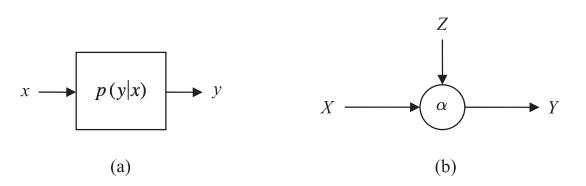
\includegraphics[width=0.5\linewidth]{imgs/exp7_2.png}
	\caption{Illustrations of (a) a discrete channel $p(y|x)$ and (b) a discrete channel $(\alpha, Z)$.}
	\label{fig:my_label}
\end{figure}
The next definition gives the condition for the equivalence of the two specifications of a discrete channel according to Definitions 7.1 and 7.2, respectively.

\begin{tcolorbox}
	\paragraph{Definition 7.3.} Two discrete channels $p(y \mid x)$ and $(\alpha, Z)$ defined on the same input alphabet $\mathcal{X}$ and output alphabet $\mathcal{Y}$ are equivalent if
	$$
	\operatorname{Pr}\{\alpha(x, Z)=y\}=p(y \mid x)
	$$
	for all $x$ and $y$
\end{tcolorbox}

\begin{tcolorbox}
	\paragraph{Definition 7.5.} $A$ discrete memoryless channel $(\alpha, Z)$ is a sequence of replicates of a generic discrete channel $(\alpha, Z) .$ These discrete channels are indexed by a discrete-time index $i,$ where $i \geq 1,$ with the ith channel being available for transmission at time i. Transmission through a channel is assumed to be instantaneous. Let $X_{i}$ and $Y_{i}$ be, respectively, the input and the output of the DMC at time $i$, and let $T_{i-}$ denote all the random variables that are generated in the system before $X_{i} .$ The noise variable $Z_{i}$ for the transmission at time $i$ is a copy of the generic noise variable $Z$ and is independent of $\left(X_{i}, T_{i-}\right) .$ The
	output of the DMC at time i is given by
	$$
	Y_{i}=\alpha\left(X_{i}, Z_{i}\right)
	$$
\end{tcolorbox}

We will prove subsequently that C is in fact the maximum rate at which
information can be communicated reliably through a DMC.
\begin{tcolorbox}
	\paragraph{Definition 7.6.} The capacity of a discrete memoryless channel $p(y \mid x)$ is defined as
	$$
	C=\max _{p(x)} I(X ; Y)
	$$
	where $X$ and $Y$ are, respectively, the input and the output of the generic discrete channel, and the maximum is taken over all input distributions $p(x)$.
\end{tcolorbox}
From the above definition, we see that $C \geq 0$
because $I(X ; Y) \geq 0$ for all input distributions $p(x)$. By Theorem 2.43 , we have
$$
C=\max _{p(x)} I(X ; Y) \leq \max _{p(x)} H(X)=\log |\mathcal{X}|
$$
Likewise, we have $C \leq \log |\mathcal{Y}|$.
Therefore,
$$
C \leq \min (\log |\mathcal{X}|, \log |\mathcal{Y}|)
$$

\subsection{The Channel Coding Theorem}
\begin{tcolorbox}
	\paragraph{Definition 7.9.} An $(n, M)$ code for a discrete memoryless channel with input alphabet $\mathcal{X}$ and output alphabet $\mathcal{Y}$ is defined by an encoding function
	$$
	f:\{1,2, \cdots, M\} \rightarrow \mathcal{X}^{n}
	$$
	and a decoding function
	$$
	g: \mathcal{Y}^{n} \rightarrow\{1,2, \cdots, M\}
	$$
	The set $\{1,2, \cdots, M\},$ denoted by $ \mathcal{W},$ is called the \textcolor{blue}{message set}. The sequences $f(1), f(2), \cdots, f(M)$ in $\mathcal{X}^{n}$ are called \textcolor{blue}{codewords}, and the set of codewords is called the \textcolor{blue}{codebook}.
\end{tcolorbox}

\begin{tcolorbox}
	\paragraph{Definition 7.10.} For all $1 \leq w \leq M,$ let
	$$
	\lambda_{w}=\operatorname{Pr}\{\hat{W} \neq w \mid W=w\}=\sum_{\mathbf{y} \in \mathcal{Y}^{n}: g(\mathbf{y}) \neq w} \operatorname{Pr}\{\mathbf{Y}=\mathbf{y} \mid \mathbf{X}=f(w)\}
	$$
	be the conditional probability of error given that the message is $w$.
	
	\paragraph{Definition 7.11.} The maximal probability of error of an $(n, M)$ code is defined as
	$$
	\lambda_{\max }=\max _{w} \lambda_{w}
	$$
	
	\paragraph{Definition 7.12.} The average probability of error of an $(n, M)$ code is defined as
	$$
	P_{e}=\operatorname{Pr}\{\hat{W} \neq W\}
	$$
\end{tcolorbox}
$$
\begin{aligned}
P_{e} &=\operatorname{Pr}\{\hat{W} \neq W\} \\
&=\sum_{w} \operatorname{Pr}\{W=w\} \operatorname{Pr}\{\hat{W} \neq W \mid W=w\} \\
&=\sum_{w} \frac{1}{M} \operatorname{Pr}\{\hat{W} \neq w \mid W=w\} \\
&=\frac{1}{M} \sum_{w} \lambda_{w} \\
&\leq \lambda_{\max }
\end{aligned}
$$

\begin{tcolorbox}
	\paragraph{Definition 7.13.} The rate of an $(n, M)$ channel code is $n^{-1} \log M$ in bits per use.
\end{tcolorbox}

\begin{tcolorbox}
	\paragraph{Definition 7.14.} A rate $R$ is asymptotically achievable for a discrete memoryless channel if for any $\epsilon>0,$ there exists for sufficiently large $n$ an $(n, M)$ code such that
	$$
	\frac{1}{n} \log M>R-\epsilon
	$$
	and
	$$
	\lambda_{\max }<\epsilon
	$$
	For brevity, an asymptotically achievable rate will be referred to as an achievable rate.
\end{tcolorbox}

\begin{tcolorbox}
	\paragraph{Theorem 7.15 (Channel Coding Theorem).} A rate $R$ is achievable for $a$ discrete memoryless channel if and only if $R \leq C,$ the capacity of the channel.
\end{tcolorbox}

\subsection{The Converse}

\begin{figure}[!h]
	\centering
	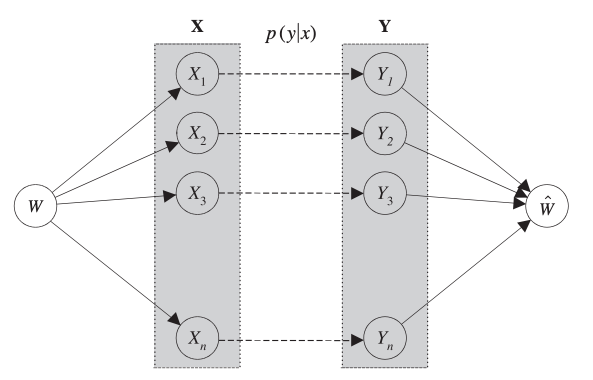
\includegraphics[width=0.5\linewidth]{imgs/exp7_9.png}
	\caption{The dependency graph for a channel code without feedback.}
	\label{fig:my_label}
\end{figure}

From the dependency graph, we see that for all $(w, \mathbf{x}, \mathbf{y}, \hat{w}) \in \mathcal{W} \times \mathcal{X}^{n} \times \mathcal{Y}^{n} \times \hat{\mathcal{W}}$
such that $q(\mathbf{x})>0$ and $q(\mathbf{y})>0$
$$
q(w, \mathbf{x}, \mathbf{y} \hat{w})=q(w)\left(\prod_{i=1}^{n} q\left(x_{i} \mid w\right)\right)\left(\prod_{i=1}^{n} p\left(y_{i} \mid x_{i}\right)\right) q(\hat{w} \mid \mathbf{y})
$$
Note that $q(w)>0$ for all $w$ so that $q\left(x_{i} \mid w\right)$ are well defined, and $q\left(x_{i} \mid w\right)$ and $q(\hat{w} \mid \mathbf{y})$ are both deterministic. Denote the set of nodes $X_{1}, X_{2}, \cdots, X_{n}$ by $\mathbf{X}$ and the set of nodes $Y_{1}, Y_{2}, \cdots, Y_{n}$ by $\mathbf{Y}$. We notice the following structure in the dependency graph: all the edges from $W$ end in $\mathbf{X},$ all the edges from $\mathbf{X}$ end in $Y,$ and all the edges from $Y$ end in $\hat{W} .$ This suggests that the random variables $W, \mathbf{X}, \mathbf{Y},$ and $\hat{W}$ form \textcolor{blue}{the Markov chain}
$$
W \rightarrow \mathbf{X} \rightarrow \mathbf{Y} \rightarrow \hat{W}
$$
The validity of this Markov chain can be formally justified by applying Proposition 2.9 to $(7.97),$ so that for all $(w, \mathbf{x}, \mathbf{y}, \hat{w}) \in \mathcal{W} \times \mathcal{X}^{n} \times \mathcal{Y}^{n} \times \hat{\mathcal{W}}$ such that
$q(\mathbf{x})>0$ and $q(\mathbf{y})>0,$ we can write
$$
q(w, \mathbf{x}, \mathbf{y}, \hat{w})=q(w) q(\mathbf{x} \mid w) q(\mathbf{y} \mid \mathbf{x}) q(\hat{w} \mid \mathbf{y})
$$
Consider a channel code whose probability of error is arbitrarily small. since $W, \mathbf{X}, \mathbf{Y},$ and $\hat{W}$ form the Markov chain in $(7.98),$ the information diagram for these four random variables is as shown in Figure $7.10 .$ Moreover, $\mathbf{X}$ is a function of $W,$ and $\hat{W}$ is a function of $\mathbf{Y} .$ These two relations are equivalent to
$H(\mathbf{X} \mid W)=0$ and $H(\hat{W} \mid \mathbf{Y})=0$
respectively. Since the probability of error is arbitrarily small, $W$ and $\hat{W}$ are essentially identical. To gain insight into the problem, we assume for the time being that $W$ and $\hat{W}$ are equivalent, so that
$$
H(\hat{W} \mid W)=H(W \mid \hat{W})=0
$$
since the $I$ -Measure $\mu^{*}$ for a Markov chain is nonnegative, the constraints in $(7.102)-(7.104)$ imply that $\mu^{*}$ vanishes on all the atoms in Figure 7.10 marked with a 0. Immediately, we see that
$$
H(W)=I(\mathbf{X} ; \mathbf{Y})
$$
That is, the amount of information conveyed through the channel is essentially the mutual information between the input sequence and the output sequence of the channel.

For a single transmission, we see from the definition of channel capacity that the mutual information between the input and the output cannot exceed the capacity of the channel, i.e., for all $1 \leq i \leq n$
$$
I\left(X_{i} ; Y_{i}\right) \leq C
$$
Summing $i$ from 1 to $n,$ we have
$$
\sum_{i=1}^{n} I\left(X_{i} ; Y_{i}\right) \leq n C
$$
\begin{tcolorbox}
	\paragraph{Lemma 7.16.} For a discrete memoryless channel used with a channel code without feedback, for any $n \geq 1$,
	$$
	I(\mathbf{X} ; \mathbf{Y}) \leq \sum_{i=1}^{n} I\left(X_{i} ; Y_{i}\right)
	$$
	where $X_{i}$ and $Y_{i}$ are, respectively, the input and the output of the channel at time $i$.
\end{tcolorbox}
Then the converse of the channel coding theorem then follows from
$$
\begin{aligned}
\frac{1}{n} \log M =\frac{1}{n} H(W) 
&=\frac{1}{n} I(\mathbf{X} ; \mathbf{Y}) \\
& \leq \frac{1}{n} \sum_{i=1}^{n} I\left(X_{i} ; Y_{i}\right) \\
& \leq C
\end{aligned}
$$

We now formally prove the converse of the channel coding theorem. Let $R$ be an achievable rate, i.e., for any $\epsilon>0,$ there exists for sufficiently large $n$ an $(n, M)$ code such that
$$
\frac{1}{n} \log M>R-\epsilon, \qquad
\lambda_{\max }<\epsilon
$$
Consider
$$
\begin{aligned}
\log M & \stackrel{a}{=} H(W) -H(W \mid \hat{W})+I(W ; \hat{W}) \\
& \stackrel{a}{\leq} H(W \mid \hat{W})+I(\mathbf{X} ; \mathbf{Y}) \\
& \leq H(W \mid \hat{W})+\sum_{i=1}^{n} I\left(X_{i} ; Y_{i}\right) \\
& \leq H(W \mid \hat{W})+n C \qquad \text{ (7.126)}
\end{aligned}
$$
where
(a) follows from (7.80)
(b) follows from the data processing theorem since $W \rightarrow \mathbf{X} \rightarrow \mathbf{Y} \rightarrow \hat{W}$
(c) follows from Lemma 7.16
(d) follows from (7.107)
From (7.87) and Fano's inequality (cf. Corollary 2.48 ), we have
$$
H(W \mid \hat{W})<1+P_{e} \log M
$$
Therefore, from (7.126)
$$
\begin{aligned}
\log M &<1+P_{e} \log M+n C \\
& \leq 1+\lambda_{\max } \log M+n C \\
&<1+\epsilon \log M+n C
\end{aligned}
$$
where we have used (7.92) and $(7.121),$ respectively, to obtain the last two inequalities. Dividing by $n$ and rearranging the terms, we have
$$
\frac{1}{n} \log M<\frac{\frac{1}{n}+C}{1-\epsilon}
$$
and from $(7.120),$ we obtain
$$
R-\epsilon<\frac{\frac{1}{n}+C}{1-\epsilon}
$$
For any $\epsilon>0,$ the above inequality holds for all sufficiently large $n .$ Let $n \rightarrow \infty$ and then $\epsilon \rightarrow 0,$ we conclude that
$$
R \leq C
$$
From the above proof, we can obtain an asymptotic bound on $P_{e}$ when the rate of the code $\frac{1}{n} \log M$ is greater than $C$. Consider (7.128) and obtain
$$
P_{e} \geq 1-\frac{1+n C}{\log M}=1-\frac{\frac{1}{n}+C}{\frac{1}{n} \log M}
$$
Then
$$
P_{e} \geq 1-\frac{\frac{1}{n}+C}{\frac{1}{n} \log M} \approx 1-\frac{C}{\frac{1}{n} \log M}
$$
when $n$ is large. This asymptotic bound on $P_{e},$ which is strictly positive if $\frac{1}{n} \log M>C$. The converse of the channel coding theorem we have proved is called the weak converse. A stronger version of this result called the strong converse can be proved, which says that $P_{e} \rightarrow 1$ as $n \rightarrow \infty$ if there exists an $\epsilon>0$ such that $\frac{1}{n} \log M \geq C+\epsilon$ for all $n$.

\newpage
\subsection{Achievability}

\begin{tcolorbox}
\paragraph{Lemma 7.17 .} Let $\left(\mathbf{X}^{\prime}, \mathbf{Y}^{\prime}\right)$ be $n$ i.i.d. copies of a pair of generic random vari-
ables $\left(X^{\prime}, Y^{\prime}\right),$ where $X^{\prime}$ and $Y^{\prime}$ are independent and have the same marginal distributions as $X$ and $Y$, respectively. Then
$$
\operatorname{Pr}\left\{\left(\mathbf{X}^{\prime}, \mathbf{Y}^{\prime}\right) \in T_{[X Y] \delta}^{n}\right\} \leq 2^{-n(I(X ; Y)-\tau)}
$$
where $\tau \rightarrow 0$ as $\delta \rightarrow 0$
\end{tcolorbox}

\begin{tcolorbox}
\paragraph{Random coding scheme}
\begin{enumerate}
	\item Construct the codebook $\mathcal{C}$ of an $(n, M)$ code randomly by generating $M$ codewords in $\mathcal{X}^{n}$ independently and identically according to $p(x)^{n} .$ Denote these codewords by $\tilde{\mathbf{X}}(1), \tilde{\mathbf{X}}(2), \cdots, \tilde{\mathbf{X}}(M)$
	\item Reveal the codebook $\mathcal{C}$ to both the encoder and the decoder.
	\item A message $W$ is chosen from $\mathcal{W}$ according to the uniform distribution.
	\item The sequence $\mathbf{X}=\tilde{\mathbf{X}}(W),$ namely the $W$ th codeword in the codebook $\mathcal{C}$ is transmitted through the channel.
	\item The channel outputs a sequence $Y$ according to 	(cf. (7.101))
	$$
	\operatorname{Pr}\{\mathbf{Y}=\mathbf{y} \mid \tilde{\mathbf{X}}(W)=\mathbf{x}\}=\prod_{i=1}^{n} p\left(y_{i} \mid x_{i}\right)
	$$
	\item The sequence $\mathbf{Y}$ is decoded to the message $w$ if $(\tilde{\mathbf{X}}(w), \mathbf{Y}) \in T_{[X Y] \delta}^{n}$ and there does not exist $w^{\prime} \neq w$ such that $\left(\tilde{\mathbf{X}}\left(w^{\prime}\right), \mathbf{Y}\right) \in T_{[X Y] \delta}^{n} .$ Otherwise, $\mathbf{Y}$ is decoded to a constant message in $\mathcal{W}$. Denote by $\hat{W}$ the message to which $\mathbf{Y}$ is decoded.
\end{enumerate}
\end{tcolorbox}
We now analyze the performance of this random coding scheme. Let
$$
E r r=\{\hat{W} \neq W\}
$$
since $\operatorname{Pr}\{\operatorname{Err} \mid W=w\}$ are identical for all $w$ by symmetry in the code construction, we have
$$
\begin{aligned}
\operatorname{Pr}\{E r r\} &=\sum_{w=1}^{M} \operatorname{Pr}\{\operatorname{Err} \mid W=w\} \operatorname{Pr}\{W=w\} \\
& = \operatorname{Pr}\{\operatorname{Err} \mid W=1\} \sum_{w=1}^{M} \operatorname{Pr}\{W=w\}  \\
& = \operatorname{Pr}\{\operatorname{Err} \mid W=1\} \\
& =\operatorname{Pr}\left\{(\tilde{\mathbf{X}}(w), \mathbf{Y}) \in T_{[X Y] \delta}^{n} \mid W=1\right\} \\
&\leq 2^{-n(I(X ; Y)-\tau)}
\end{aligned}
$$

$$
\operatorname{Pr}\{E r r\}<\frac{\epsilon}{2}
$$
Thus by discarding the worse half of the codewords in $\mathcal{C}^{*},$ for the resulting codebook, the maximal probability of error $\lambda_{\max }$ is less than $\epsilon .$ Using (7.183) and considering
$$
\begin{aligned}
\frac{1}{n} \log \frac{M}{2} &=\frac{1}{n} \log M-\frac{1}{n} \\
&>\left(I(X ; Y)-\frac{\epsilon}{2}\right)-\frac{1}{n} \\
&>I(X ; Y)-\epsilon
\end{aligned}
$$
when $n$ is sufficiently large, we see that the rate of the resulting code is greater than $I(X ; Y)-\epsilon .$ Hence, we conclude that the rate $I(X ; Y)$ is achievable.

\subsection{A Discussion}
\subsection{Feedback Capacity}

\begin{tcolorbox}
\paragraph{Definition 7.18.} An $(n, M)$ code with complete feedback for a discrete memoryless channel with input alphabet $\mathcal{X}$ and output alphabet $\mathcal{Y}$ is defined by encoding functions
$$
f_{i}:\{1,2, \cdots, M\} \times \mathcal{Y}^{i-1} \rightarrow \mathcal{X}
$$
for $1 \leq i \leq n$ and a decoding function
$$
g: \mathcal{Y}^{n} \rightarrow\{1,2, \cdots, M\}
$$
\end{tcolorbox}
\begin{tcolorbox}
\paragraph{Definition 7.19.} $A$ rate $R$ is achievable with complete feedback for a discrete memoryless channel $p(y \mid x)$ if for any $\epsilon>0,$ the re exists for sufficiently large $n$ an $(n, M)$ code with complete feedback such that
$$
\frac{1}{n} \log M>R-\epsilon
$$
and
$$
\lambda_{\max }<\epsilon
$$
\end{tcolorbox}
\begin{tcolorbox}
\paragraph{Definition 7.20.} The feedback capacity, $C_{F B},$ of a discrete memoryless channel is the supremum of all the rates achievable by codes with complete feedback.\\

\paragraph{Proposition 7.21.} The supremum in the definition of $C_{F B}$ in Definition 7.20 is the maximum.
\end{tcolorbox}

\begin{tcolorbox}
Lemma $7.22 .$ For all $1 \leq i \leq n$
$$
\left(W, \mathbf{Y}^{i-1}\right) \rightarrow X_{i} \rightarrow Y_{i}
$$
forms a Markov chain.
\end{tcolorbox}
\subsection{Separation of Source and Channel Coding}
This result, sometimes called the \emph{separation theorem for source and channel coding}, says that asymptotic optimality can be achieved by separating source coding and channel coding. This theorem has significant engineering implication because the source code and the channel code can be designed separately without losing asymptotic optimality. Specifically, we only need to design the best source code for the information source and design the best channel code for the channel. Moreover, separation of source coding and channel coding facilitates the transmission of different information sources on the same channel because we need only change the source code for different in- formation sources. Likewise, separation of source coding and channel coding also facilitates the transmission of an information source on different channels because we need only change the channel code for different channels.Likewise, separation of source coding and channel coding also facilitates the transmission of an information source on different channels because we need only change the channel code for different channels.
\end{document}